\documentclass[11pt,a4paper]{book}
\synctex=1
\usepackage[italian]{babel}
\usepackage{acronym}
\usepackage{graphicx}
\usepackage{amsmath}
\usepackage{amsfonts}
\usepackage{amssymb}
\usepackage{psfrag}
\usepackage{listings}
\usepackage{url}
\usepackage{setspace}
\usepackage{cmap}
\usepackage{hyperref}
\hypersetup{
    colorlinks,%
    citecolor=black,%
    filecolor=black,%
    linkcolor=black,%
    urlcolor=black
}
\usepackage{breakurl}
% interlinea 1.5
\onehalfspace


\begin{document}
%----------------------------------------------------------
%	Fronte - Sommario - Varie
%----------------------------------------------------------
%!TEX root = ../tesi.tex
\tableofcontents
\listoffigures
\listoftables
%!TEX root = ../tesi.tex
\chapter*{Acronimi}

\begin{acronym}[GPU]

	\acro{SF}{Shadow Framework}
	\acro{GPU}{Graphic Processing Unit}

\end{acronym}



%----------------------------------------------------------
%	Capitoli
%----------------------------------------------------------
%!TEX root = ../tesi.tex

\chapter{Introduzione}
\label{ch:introduzione}
La presente tesi si colloca nell'ambito dello sviluppo dello \ac{SF} 2.0, un framework concepito per la realizzazione di applicazioni che fanno uso di grafica tridimensionale real-time ideato e sviluppato dall'Ingegner Alessandro Martinelli.

La grafica tridimensionale, o computer grafica 3D, consiste nell'utilizzo di modelli geometrici tridimensionali da parte di un computer per il calcolo e il rendering\footnote{Con rendering, in computer grafica, si intende il processo che attraverso l'elaborazione di un modello determina il colore di ogni pixel contenuto in una immagine digitale\cite{wiki:rendering-it,wiki:rendering-en}.} di immagini digitali.

Essa \`e attualmente diffusa in molteplici campi, cosa che la rende un'esperienza comune nella vita di tutti giorni. Non solo infatti viene utilizzata in modo intensivo nella pubblicit\`a e nell'intrattenimento ma anche in settori come quello medico e nella ricerca scientifica.

La grafica tridimensionale real-time \`e un ramo specifico della grafica tridimensionale che si focalizza sulla generazione di simulazioni di ambienti e/o oggetti con la quale un utente pu\`o interagire osservando una reazione coerente nella simulazione. Questa percezione di interazione viene fornita da una generazione sequenziale di immagini che come nelle pellicole cinematografiche danno un'illusione di movimento, ma in cui l'effettivo contenuto dei fotogrammi non \`e predeterminato ed \`e calcolato al momento sulla base degli input forniti.

In base a quanto esplicato in \cite{book:realtimerendering}, per poter avere un'interazione soddisfacente \`e molto importante che la velocit\`a con cui vengono visualizzate le immagini, misurata in \ac{fps}, si mantenga stabile ed il pi\`u possibile elevata in modo da minimizzare i tempi di risposta ed impedire che questi interferiscano con l'interazione stessa.
Ci\`o pone il problema di ottenere un alto valore di \ac{fps} che a sua volta implica dei vincoli temporali sulla possibile elaborazione dei modelli tridimensionali: se per esempio si volesse mantenere una velocit\`a di visualizzazione pari a 60 \ac{fps}, il tempo di calcolo a disposizione per l'elaborazione di un frame rispetto al precedente ammonterebbe a circa 15 millisecondi.
Questa caratteristica differenzia profondamente la grafica real-time da quella non-real-time in cui, non avendo vincoli temporali stretti per la generazione dei frame, il focus \`e spostato sull'applicazione di modelli di elaborazione complessi e computazionalmente onerosi che siano in grado di generare immagini il pi\`u fotorealistiche possibile. 

Le problematiche della grafica real-time hanno imposto nel corso degli anni lo sviluppo di tecniche e tecnologie specifiche di settore il cui stato dell'arte \`e oggi rappresentato dall'ultima generazione di \ac{API} di programmazione grafica, dalle \ac{GPU}\footnote{Una \ac{GPU} \`e un microprocessore dedicato alla generazione delle immagini visualizzate sullo schermo di un dispositivo, alleggerendo da questo carico il processore principale.} a pipeline programmabile e dai Linguaggi di Shading.

Queste tecnologie hanno assunto una grande importanza perch\'e consentono di raggiungere elevatissimi livelli di qualit\`a e prestazioni quando sono utilizzate per la generazione di grafica 3D real-time e la ricerca su di esse ha portato allo sviluppo del \ac{GPGPU} ovvero la possibilit\`a di utilizzare la capacit\`a di calcolo delle \ac{GPU} per processare anche dati differenti da quelli grafici.

Le \ac{GPU} a pipeline programmabile, in contrapposizione a quelle con pipeline fissa, permettono di adattare gli stadi della pipeline di renderizzazione mediante l'utilizzo dei linguaggi di Shading. In sostanza l'hardware viene programmato per il calcolo di algoritmi specifici da applicare ai dati grafici. Ci\`o consente di adattare il processo di renderizzazione agli effetti che si desidera ottenere e di sfruttare l'hardware della \ac{GPU} per velocizzarne la computazione. 
Questo paradigma si \`e rivelato molto efficace ed efficiente, tanto da venire oggi applicato nella quasi totalit\`a delle \ac{GPU} moderne, sia che si tratti di dispositivi di fascia alta che di processori grafici dedicati ad architetture mobile come i cellulari.

Parallelamente le \ac{API} di programmazione grafica moderne si sono sviluppate consentendo lo sfruttamento sempre pi\`u efficiente delle risorse hardware delle \ac{GPU}, ma non solo: la loro integrazione su piattaforme software pensate per il mercato embedded ha consentito una proliferazione di applicazioni che fanno uso di grafica tridimensionale sia su cellulari che tablet.
Non \`e difficile trovare per questi dispositivi, dotati ormai quasi obbligatoriamente di fotocamera, applicazioni di realt\`a aumentata che sfruttino le \ac{API} per inserire elementi grafici tridimensionali nelle immagini catturate dal sensore ottico.
Un evento che nei prossimi anni porter\`a un impatto significativo sul mercato, consiste nel fatto che molti sviluppatori di browser per la navigazione di internet stanno attualmente lavorando per integrare l'\ac{API} grafica WebGL all'interno dei loro software tramite JavaScript. Questo consentir\`a l'esecuzione di applicazioni 3D direttamente all'interno dei browser stessi, eliminando la transizione tra contenuti 3D e contenuti non-3D e consentendo una integrazione diretta con servizi internet di terze parti.

Di pari passo, i produttori di middleware, engine e framework\footnote{Nel contesto delle applicazioni per la grafica tridimensionale con middleware di solito si intendono componenti software dedicate a compiti specifici, come la gestione della fisica o il pathfinding, che vengono affiancate agli engine ed ai framework. Per una descrizione pi\`u completa di engine e framework e le differenze fra loro, fare riferimento alla sezione \ref{sec:panoramicastrumenti}}, hanno integrato nelle funzionalit\`a dei loro prodotti la capacit\`a di sfruttare le pipeline programmabili e tool per testare e comporre nuovi shader\footnote{Uno shader \`e un programma scritto con un linguaggio di shading, che viene caricato ed eseguito in hardware da una \ac{GPU}.}. Una sempre maggiore quantit\`a di queste case produttrici supportano le piattaforme mobile (come Android e iOS) e rilasciano plugin o applicazioni ``WebPlayer'' per distribuire contenuti attraverso i browser web. 
In alcuni casi, come quello citato in \cite{site:mozillaunrealannounce}, produttori di browser e case di sviluppo collaborano per migliorare le prestazioni di WebGL e convertire in JavaScript gli engine e i framework cos{\`\i} da poterli eseguire direttamente all'interno delle pagine web.

In questo contesto si inserisce lo Shadow Framework, il quale \`e stato progettato non solo per utilizzare e supportare tutte le tecnologie che costituiscono lo stato dell'arte nel campo della grafica 3D real-time, ma anche con l'obbiettivo di farlo sperimentando un nuovo approccio nella generazione e nella gestione dei dati grafici tridimensionali. 
La chiave di questo approccio consiste nell'abbandonare la vecchia concezione per cui gli oggetti tridimensionali sono scolpiti generando mesh di vertici che compongono triangoli, ma utilizzando primitive parametriche pi\`u complesse per poi sfruttare le capacit\`a delle pipeline programmabili e far generare dall'hardware stesso le mesh di punti necessarie per il processo di renderizzazione.
Questo tipo di procedimento permette di adattare la qualit\`a  del risultato visivo finale in base alle prestazioni dell'hardware a disposizione, eliminando la necessit\`a di produrre diverse versioni dello stesso modello la cui unica differenza consiste nel numero di vertici. \`E infatti sufficiente programmare la pipeline per produrre un minor numero di vertici per alleggerire il calcolo, mantenendo inalterato il modello parametrico di partenza.

Oltre ai vantaggi descritti, l'utilizzo di primitive parametriche permette di produrre file di dimensione molto contenuta rispetto ai sistemi classici in cui i file contengono l'elenco dei vertici che descrivono l'oggetto. Lo stesso paradigma viene usato all'interno del framework non solo per i modelli 3D, ma anche per la generazione delle texture da applicarvi, garantendo un meccanismo per scalarne la qualit\`a in base alle esigenze.

Le caratteristiche principali del framework, la cui spiegazione pi\`u dettagliata verr\`a esposta nel capitolo  \ref{ch:shadowframework}, sono le seguenti:
\begin{itemize}
	\item  la possibilit\`a di definire nuove primitive grafiche con un linguaggio specifico del framework;
	\item  la grande portabilit\`a: la versione di riferimento \`e sviluppata in linguaggio Java, ma \`e in corso di realizzazione un porting in C++ (iOS);
	\item  il design web-oriented: i meccanismi interni sono stati progettati per supportare l'utilizzo di dati in remoto ed \`e in corso di realizzazione una versione del framework in JavaScript;
\end{itemize}

%
% TODO: DA RIVEDERE, deve essere chiaro che l'applicativo voluto deve essere orientato al web
%
\section{Obbiettivo del progetto}
\label{sec:obbiettivo}
L'obbiettivo del progetto di tesi nasce dall'idea di produrre un'applicazione dimostrativa delle funzionalit\`a di rete offerte dallo Shadow Framework.
Ci\`o che si voleva ottenere era una coppia client-server in cui il server fosse in grado di gestire connessioni simultanee da parte di un numero indefinito di client. 
Ogni client, ottenuta una connessione con il server, doveva poter visualizzare una scena iniziale navigabile, richiedendo solamente i dati relativi all'ambiente in prossimit\`a della posizione, all'interno della scena, dell'utente.

Successivamente si volevano analizzare due possibili approcci: il primo in cui il client richiede al server i dati aggiuntivi riguardo la scena a seconda delle necessit\`a, ad esempio una volta raggiunti i bordi dell'ambiente. Nel secondo il server tiene traccia degli spostamenti nella navigazione comunicando attivamente con il client, componendo in modo dinamico dei pacchetti di dati che prevedano le future richieste del client.

Le astrazioni del layer dati del framework sono state progettate specificatamente per consentire lo sfruttamento della comunicazione di rete, ma fino a quel momento non era stata fatta alcuna specifica implementazione che la utilizzasse. Si desiderava perci\`o produrre questo tipo di applicazione non solo a scopo dimostrativo, ma anche per individuare e correggere probabili bug presenti nel codice e dovuti a vincoli di sincronizzazione non evidenziati dai test effettuati con dati memorizzati su macchina locale.

L'obbiettivo della tesi \`e cos{\`\i} diventato quello di produrre dei moduli di libreria che fossero utili allo sviluppo di applicazioni client-server.

La progettazione di questi moduli si \`e focalizzata su alcuni punti cardine che rappresentano la chiave dello sviluppo del progetto. La struttura del framework \`e stata ideata con l'obbiettivo di garantirne l'estendibilit\`a, perci\`o \`e stato di fondamentale importanza sfruttare i meccanismi e le astrazioni previste in tal senso e lo sviluppo dei moduli \`e stato guidato dagli stessi principi.

\section{Organizzazione del documento}
\label{sec:orgtesi}
Il presente documento \`e organizzato secondo la seguente suddivisione in capitoli:
\begin{itemize}
	\item  \textbf{Capitolo \ref{ch:shadowframework}:} in cui viene presentata una panoramica generale sullo Shadow Framework 2.0 in rapporto al panorama generale sui framework di programmazione di grafica tridimensionale real-time.
	\item  \textbf{Capitolo \ref{ch:gestionedati}:} in cui \`e descritta l'astrazione di gestione dei dati interna al framework e come essa viene utilizzata dalle applicazioni \ac{SF}.
	\item  \textbf{Capitolo \ref{ch:sfremoteconnection}:} in cui viene descritto il progetto Sf-Remote-Connection, i moduli che lo compongono, le funzionalit\`a offerte e i package java prodotti.
	\item  \textbf{Capitolo \ref{ch:testerisultati}:} in cui sono presentate le applicazioni di test ed i risultati prodotti.
	\item  \textbf{Capitolo \ref{ch:conclusioni}:} in cui viene presentato un riassunto del lavoro svolto, i risultati e vengono proposti alcuni sviluppi futuri.
\end{itemize}



%!TEX root = ../tesi.tex

\chapter{Lo Shadow Framework 2.0}
\label{ch:shadowframework}
Questo capitolo presenta inizialmente una panoramica sugli attuali sistemi per la realizzazione di applicazioni che fanno uso di grafica tridimensionale real-time. Successivamente viene presentato lo ShadowFramework 2.0, le sue caratteristiche, la sua struttura e i suoi sviluppi futuri.

\section{Panoramica sui framework per la grafica 3D interattiva}
\label{sec:panoramicastrumenti}
Lo scopo della presente tesi di laurea \`e quello di produrre dei moduli di estensione per lo Shadow Framework, utili alla realizzazione di applicativi 3D orientati al web. 
Per lo stesso scopo esistono sul mercato una grande quantit\`a di soluzioni le cui caratteristiche possono essere notevolmente differenti in base al target di sviluppo a cui si rivolgono.

Prima di fornire una descrizione di alcune di queste soluzioni \`e bene introdurre alcuni concetti utili a comprendere quali sono i punti focali che distinguono un prodotto da un altro. L'elemento fondamentale di ognuno di questi questi software \`e l'\textbf{engine}, altrimenti detto rendering engine o 3D-engine. Questo \`e il nucleo di ogni programma grafico e fornisce una serie di meccanismi che, sfruttando le \ac{API} di programmazione grafica, permettono di disegnare su schermo i modelli tridimensionali voluti. Quando un prodotto consiste nel solo engine viene fornito nella forma di una libreria con cui \`e possibile interagire attraverso una \ac{API} specifica e che permette di configurare i passaggi della fase di rendering.

Dato che la pi\`u grande fetta di mercato per queste soluzioni software proviene dallo sviluppo di videogames sono nati una serie di software definiti \textbf{game engine}, questi sono veri e propri framework per la produzione di applicazioni 3D e, oltre al rendering engine, integrano al loro interno moduli per la gestione della fisica, del suono, delle animazioni e di tutte quelle componenti utili per lo sviluppo di giochi per computer. Questi framework possono essere forniti sia sotto forma di libreria da integrare nel proprio codice che con tool grafici che permettono di creare la propria applicazione da zero, utilizzando solamente gli strumenti forniti.

Seguendo questa classificazione e dato che l'intento dello Shadow Framework \`e fornire un set di librerie completo per la creare applicazioni grafiche, con moduli per gestire animazioni e dati oltre che alla semplice renderizzazione, senza per\`o vincolare all'utilizzo di librerie specifiche per elementi come l'intelligenza artificiale, il suono o altro che non sia direttamente coinvolto nella gestione della grafica, esso si trova a met\`a strada tra un rendering engine puro e un game engine.

Vengono ora presentati alcuni dei prodotti presenti sul mercato, la scelta di quali di essi presentare rispetto ad altri che non verranno citati non riflette la loro qualit\`a, ma \`e stata fatta su base rappresentativa.

% TODO: inserire i simboli di copyright ecc
\subsection{Game engine per Adobe Flash}
In questo caso invece che un prodotto specifico si preferisce citare una categoria di software. Per l'ambiente di Adobe esistono una grande quantit\`a di game engine che sfruttano le \ac{API} Flash per effettuare il rendering dei contenuti. Sebbene questo framework venga utilizzato da molti anni per la realizzazione di applicativi e che per lungo tempo abbia rappresentato l'ambiente di riferimento per applicativi web 3D, solo dalla release 11 comincia a sfruttare l'accelerazione hardware per la grafica tridimensionale.

Attualmente l'accelerazione consente di sfruttare le GPU a pipeline programmabile, ma non consente di usare le modalit\`a legacy a pipeline fissa. 
Inoltre non vengono rese disponibili le \ac{API} grafiche per la programmazione nativa come OpenGL o DirectX, ma una \ac{API} proprietaria di nome Stage3D che fornisce un'astrazione di livello pi\`u alto e semplifica la gestione delle risorse.
Questo sebbene consenta di semplificare e unificare tutte le piattaforme compatibili rende necessarie delle limitazioni per conservare la compatibilit\`a, rendendo inaccessibili le funzionalit\`a pi\`u avanzate degli hardware moderni (ad esempio \`e supportato lo Shader Model solo fino alla versione 2.0 sebbene oggi sia disponibile la versione 5.0).
Questi dati sono reperiti da \cite{site:adobestage3d}.

\subsection{Unity 3D}
Unity 3D \`e un game engine completo che dal 2005 ad oggi ha accresciuto molto la sua popolarit\`a. Uno dei maggiori punti di forza di questo ambiente consiste nella presenza di una discreta quantit\`a di tool grafici integrati tra loro, per il controllo del workflow di sviluppo. Sono inoltre integrati molti moduli per controllare aspetti quali le animazioni, la verifica delle performance ed il networking.
Un qualit\`a di primo piano \`e la compatibilit\`a di un elevato numero di piattaforme, consentendo di pubblicare le applicazioni realizzate su piattaforme mobile (android e iOS), desktop (Windows, Mac e Linux), console e web (via browser).
A proposito di quest'ultimo caso la fruizione dei contenuti via web \`e effettuata con due diversi metodi: o tramite un player flash o tramite l'\ac{API} Google Native Client del browser Chrome che permette l'esecuzione di codice nativo all'interno del browser.
In generale Unity 3D \`e un game engine moderno con pieno supporto alle ultime tecnologie grafiche rendendolo uno prodotto molto rappresentativo.
Oltre alle caratteristiche citate buona parte del suo successo \`e probabilmente dovuto alla grande comunit\`a di sviluppatori, anche indipendenti, ed alla numerosa quantit\`a di asset grafici disponibili.

\subsection{Unreal Engine e Unigine engine}
Entrambi questi prodotti sono game engine completi piuttosto famosi per l'elevatissima qualit\`a delle loro capacit\`a di rendering. Entrambi vengono infatti spesso utilizzati come benchmark per testare le capacit\`a grafiche hardware. Entrambi questi progetti sono maturi e moderni essendo dotati di tool grafici specifici e supportando le pi\`u recenti architetture grafiche. Entrambi supportano la maggior parte delle piattaforme desktop, mobile e consolle. Sebbene l'Unreal engine supporti anche flash e l'Unigine no, sono presentati insieme in quanto esempio di nuovo approccio alla distribuzione via web: entrambe le compagnie produttrici di questi software stanno infatti investendo nel portare i loro framework a supportare \ac{API} WebGL. Gli annunci ufficiali possono essere trovati a questi riferimenti \cite{site:mozillaunrealannounce,site:unigineannounce}.

\subsection{OnLive e Gaikai}
I due citati nel titolo non sono software per produrre applicazioni di grafica, ma due servizi a pagamento per la fruizione di applicazioni e videogiochi attraverso lo streaming online e vengono qui citati come esempio di una tecnologia alternativa per la fruizione di contenuti basati su grafica 3D real-time. 

Entrambe le soluzioni eseguono su richiesta le applicazioni su server proprietari e all'utente viene fornito di un client, hardware o software, che attraverso una connessione ad internet permette di ricevere l'output video del server mediante un video in live streaming. Il client si occupa inoltre di intercettare l'input dell'utente e inviarlo ai server che stanno eseguendo l'applicazione in modo che possano processarlo per rendere interattiva la fruizione del servizio.

L'utilizzo di questo approccio consente all'utente di non doversi dotare di dispositivi hardware dall'elevata potenza di calcolo dato che il peso della computazione della grafica \`e totalmente a carico dei server. In questo caso il punto focale che influenza la qualit\`a dell'interazione consiste nelle prestazioni della connessione di rete, che deve essere continuata, con una elevata larghezza di banda e mantenere una bassa latenza.
Informazioni relative a questi servizi sono reperibili tramite \cite{site:onlive,site:gaikai}.

\section{Introduzione allo Shadow Framework 2.0}
\label{sec:sfintro}
Le tecnologie della pipeline di rendering programmabile e delle \ac{API} 3D, tra cui lo standard pi\`u diffuso \`e OpenGL, hanno avuto una notevole influenza sull'industria della produzione di applicazioni di grafica tridimensionale, ma un impatto altrettanto significativo si \`e verificato anche nel campo della ricerca in cui, grazie ad esse, si \`e raggiunto lo sviluppo di numerose soluzioni innovative e la generazione di effetti che senza l'ausilio delle suddette tecnologie, erano impossibili da implementare.
Nonostante la bont\`a di molte di queste ricerche, solamente una parte di esse ha effettivamente trovato un'applicazione nel mondo dell'industria di settore e anche in quel caso la loro applicazione \`e stata indirizzata ad un miglioramento delle tecniche e delle consuetudini definite negli anni piuttosto che ad un rinnovamento radicale.

L'obbiettivo fondamentale dichiarato per lo Shadow Framework \`e proprio quello di ridefinire l'architettura classica delle applicazioni di grafica attraverso l'utilizzo dei nuovi paradigmi consentiti dalla nuova tecnologia: ``Noi sosteniamo che cambiare si pu\`o. La tecnologia \`e matura quanto basta per sperimentare soluzioni alternative che siano pi\`u in linea con le tecnologie moderne e che siano in grado di rispondere in modo migliore alle esigenze del Web 3D''\cite{site:shadowframework}.

Per meglio comprendere l'approccio innovativo sperimentato dal framework dobbiamo individuare dove e perch\'e un'applicazione di questo tipo utilizza al suo interno i dati grafici tridimensionali e qual'\`e l'impatto che ognuno di questi ``momenti'' ha sulla responsivit\`a del sistema.

\subsection{I tre ``momenti'' di utilizzo dei dati}
``Nei casi pratici ogni applicazione che fa uso della grafica tridimensionale passa per tre momenti molto importanti: \textbf{accesso} ai dati tridimensionali, la fase di \textbf{costruzione e inizializzazione} e la \textbf{visualizzazione}''\cite{site:shadowframework}.

Con \textbf{accesso} ai dati tridimensionali si intende il caricamento dei dati in memoria ram. In un'applicazione tradizionale questi dati sono memorizzati all'interno di file gi\`a presenti sulla memoria di massa locale, per questo motivo il loro caricamento non \`e mai considerato critico per quanto riguarda le prestazioni e la responsivit\`a nonostante la dimensione di questi dati spesso raggiunge le decine di giga byte. 

La fase di \textbf{construzione e inizializzazione} consiste in quel processo in cui i dati caricati da file devono essere usati per costruire nella memoria grafica le strutture dati effettivamente utilizzabili dalle \ac{GPU}, non \`e raro che per esaudire questo compito le informazioni abbiano la necessit\`a di essere trasformate o decompresse per essere adattate alle suddette strutture.
In alcuni casi, specialmente per dati di grosse dimensioni, questa inizializzazione viene svolta una sola volta all'inizio e prima di cominciare la visualizzazione.

La \textbf{visualizzazione} \`e quella fase in cui i dati grafici, caricati e inizializzati nella memoria grafica vengono processati per produrre i fotogrammi della sequenza che si desidera produrre.

Storicamente, e non senza motivo, il processo di visualizzazione \`e quello su cui si sono concentrati i maggiori sforzi sia per quanto riguarda la ricerca di una maggiore qualit\`a visiva, sia per quanto concerne la reattivit\`a delle applicazioni. Queste due componenti sono parte di un complesso equilibrio che cerca di bilanciare il tempo di calcolo concesso al processo di rendering e i tempi stretti concessi alla produzione di un singolo frame per garantire una fruizione fluida e interattiva. Va fatto notare che nel tempo che intercorre tra un frame e l'altro non deve essere eseguito il solo processo di rendering, ma deve anche essere applicato l'input dell'utente e in alcuni casi applicata una simulazione fisica e l'intelligenza artificiale di agenti interni alla simulazione.

\begin{figure}
\begin{center}
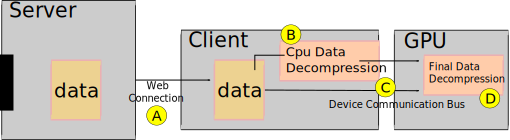
\includegraphics[width=\textwidth]{Immagini/genericdecompressionpipeline}
\caption[Schema agenti della distribuzione dei dati]{Schema degli agenti coinvolti nella distribuzione dei dati tridimensionali via rete. Sono posti in evidenza: A)la connessione di rete attraverso cui client e server comunicano; B)la ``decompressione'' effettuata, se necessario, dalla cpu del client; C)il bus di comunicazione tra la memoria principale e la memoria della GPU; D)l'eventuale e ulteriore ``decompressione'' effettuata dalla GPU stessa.\label{f:genericdecompressionpipeline}} 
\end{center} 
\end{figure}

\subsection{Applicazioni orientate al Web 3D}
Con la diffusione di applicazioni web 3D questa prospettiva \`e destinata per\`o a cambiare dato che per i sistemi tradizionali l'utilizzo di una grande quantit\`a di dati rende non pi\`u trascurabili i tempi di reperimento e caricamento. 
Per ovviare a questo problema, le soluzioni pi\`u diffuse sono una, a volte drastica, diminuzione della qualit\`a visiva o al rilascio di client che necessitano di installazione da parte dell'utente e che memorizzano in locale tutti i dati grafici. Quest'ultimo metodo \`e probabilmente il pi\`u diffuso per tutte quelle applicazioni che puntano ad avere sia elevata qualit\`a visiva che interazione tra utenti remoti, ma \`e anche quello che si separa di pi\`u dalle caratteristiche del web.
L'approccio del framework \`e invece quello di affrontare il problema aumentando la criticit\`a delle fasi di \textbf{accesso}, \textbf{costruzione e inizializzazione}.

Se si analizzano le applicazioni di grafica distribuite sulla rete, si pu\`o risalire a tre moduli distinti che sono di interesse: il server, il client e l'acceleratore grafico a disposizione del client. I dati contenuti sul server, per essere utilizzati, devono arrivare all'acceleratore grafico nella forma delle strutture dati proprie di quest'ultimo. Escludendo l'approccio a client con dati grafici autonomi possiamo modellizzare questo scenario come mostrato nella figura \ref{f:genericdecompressionpipeline}, in essa possiamo vedere in ordine temporale da sinistra a destra, il percorso fisico attraversato dai dati. Questi partono dal server e viaggiano attraverso una connessione web (A) fino a raggiungere il client, qui vengono caricati in memoria ed eventualmente ``decompressi'' dalla cpu (B), successivamente vengono inviati alla memoria video attraverso il bus di connessione della scheda grafica (C) ed infine, prima di essere visualizzati, possono dover attraversare un ulteriore processo di elaborazione/decompressione da parte della \ac{GPU} stessa (D). \`E facile identificare nella connessione (A) il collo di bottiglia del sistema, dato che in esso la banda a disposizione per il trasferimento dati \`e in assoluto la pi\`u piccola e non consente di sfruttare pienamente le capacit\`a di calcolo della \ac{GPU}.

Le applicazioni tradizionali si limitano ad utilizzare strutture dati datate, solitamente basate sulle mesh di vertici\footnote{Le mesh di vertici, o mesh poligonali, rappresentano i modelli tridimensionali attraverso un elenco di punti che definiscono i vertici di figure poligonali, di solito triangoli, in uno spazio tridimensionale.}, che per le loro caratteristiche producono file di grosse dimensioni, pi\`u che sufficienti nel caso in cui i dati sono memorizzati in locale, ma poco adeguati ad un contesto di comunicazione remota. I file vengono trasferiti attraverso il canale (A), il client se necessario effettua in (B) una decompressione dei dati e carica in memoria le informazioni contenute , nello stadio (C) i dati vengono trasferiti nella memoria video all'interno di strutture dati adatte a seconda del caso. Una volta all'interno della memoria della \ac{GPU} di solito i dati non vengono ulteriormente processati prima della visualizzazione, ma tutti gli ulteriori effetti vengono aggiunti durante il rendering stesso.

Dato il collo di bottiglia della connessione web (A) \`e proprio la dimensione dei file a rappresentare il maggiore limite del sistema. Per questo motivo \`e consuetudine che anche le applicazioni che non usano client con dati grafici preinstallati dedichino una fase iniziale ad effettuare il download completo di tutti i dati.

Le applicazioni basate sul modello del live streaming hanno problemi simili: in questo caso si ha il trasferimento attraverso (A) dei dati del flusso video, la banda occupata da questo flusso per livelli di qualit\`a medio-alta pu\`o variare da pochi Mbit/s alle decine di Mbit/s. Le informazioni video hanno bisogno di un solo stadio di decompressione che pu\`o essere effettuato sia direttamente dalla cpu in (B) che all'interno di processori grafici che implementano i decoder specifici, ma la \ac{GPU} vera e propria non viene affatto utilizzata. Come gi\`a accennato il vantaggio di ci\`o consiste nel fatto che il client non necessita affatto di avere a disposizione una \ac{GPU} e non vi \`e necessit\`a perci\`o di memorizzare i dati grafici. Gli svantaggi sono che vi \`e la necessit\`a di una connessione costante anche quando vengono visualizzati oggetti precedentemente visti e che la qualit\`a non \`e influenzata dall'hardware a disposizione, ma solo dalla banda a disposizione.

In entrambe le situazioni analizzate la possibilit\`a offerte dallo stadio (D) non vengono sfruttate ed \`e proprio tramite il suo utilizzo che lo Shadow Framework cerca di risolvere il problema. Facendo riferimento alla figura \ref{f:genericdecompressionpipeline}, sul server sono memorizzati i dati modellizzati in una forma parametrica adatta ad essere processata dalla \ac{GPU}: si pensi ad esempio ad una sfera descritta dalla posizione del proprio centro e dal suo raggio, utilizzando l'equazione parametrica della sfera \`e possibile calcolare dinamicamente in un secondo tempo la mesh di vertici che approssima il modello. Questa forma di ``decompressione'' dei dati consente di alleggerire i modelli contenuti nei file dal compito di trasportare al loro interno molte informazioni in maniera esplicita in maniera simile a quanto avviene ai formati vettoriali per le immagini bidimensionali. I file possono perci\`o essere di dimensioni contenute, diminuendo sensibilmente il tempo di \textbf{accesso} ai dati e scaricando parte del processo di reperimento delle informazioni anche sulla fase di \textbf{costruzione e inizializzazione} eseguita sulla \ac{GPU} stessa.

\subsection{Funzionalit\`a avanzate}
Alla luce del principio esposto al precedente paragrafo si pu\`o giungere successivamente ad ulteriori rielaborazioni di diverse pratiche sfruttate attualmente dai framework e dalle applicazioni grafiche. Una di queste pratiche \`e l'utilizzo della \textbf{precomputazione}, ovvero il processo di pre-calcolare dati computazionalmente troppo onerosi per essere gestiti in real-time. Questa precomputazione pu\`o essere eseguita in fase di inizializzazione di un'applicazione oppure essere effettuati a monte e memorizzati in modo statico in file la cui dimensione pu\`o rivelarsi. 

In contesto web la seconda soluzione \`e la meno conveniente dato che aumenta la quantit\`a di dati da trasferire attraverso il canale di comunicazione, ma alla luce dei moderni hardware grafici in generale anche la prima pu\`o essere ripensata sia nel senso di limitarla che nel senso di spostarne il peso computazionale direttamente sulla \ac{GPU}.

Un'altra interessante considerazione riguarda la valutazione del livello di dettaglio: le applicazioni tradizionali per adattare la qualit\`a delle immagini prodotte alla potenza dell'hardware a disposizione ricorrono all'espediente di fornire differenti varianti della stessa risorsa grafica a diversi livelli di qualit\`a. Per il rendering della stessa scena sono perci\`o disponibili modelli tridimensionali con un diverso numero di vertici o varianti della stessa immagine a diverse risoluzioni. Questo consente di alleggerire il calcolo su \ac{GPU} meno potenti, ma dato che aumenta notevolmente la dimensione dei dati \`e una soluzione insoddisfacente nel contesto web. L'utilizzo di una modellizzazione gerarchica all'interno del framework fornisce un meccanismo alternativo per gestire il livello di dettaglio che non va ad impattare sulla dimensione dei dati.

\begin{figure}
\begin{center}
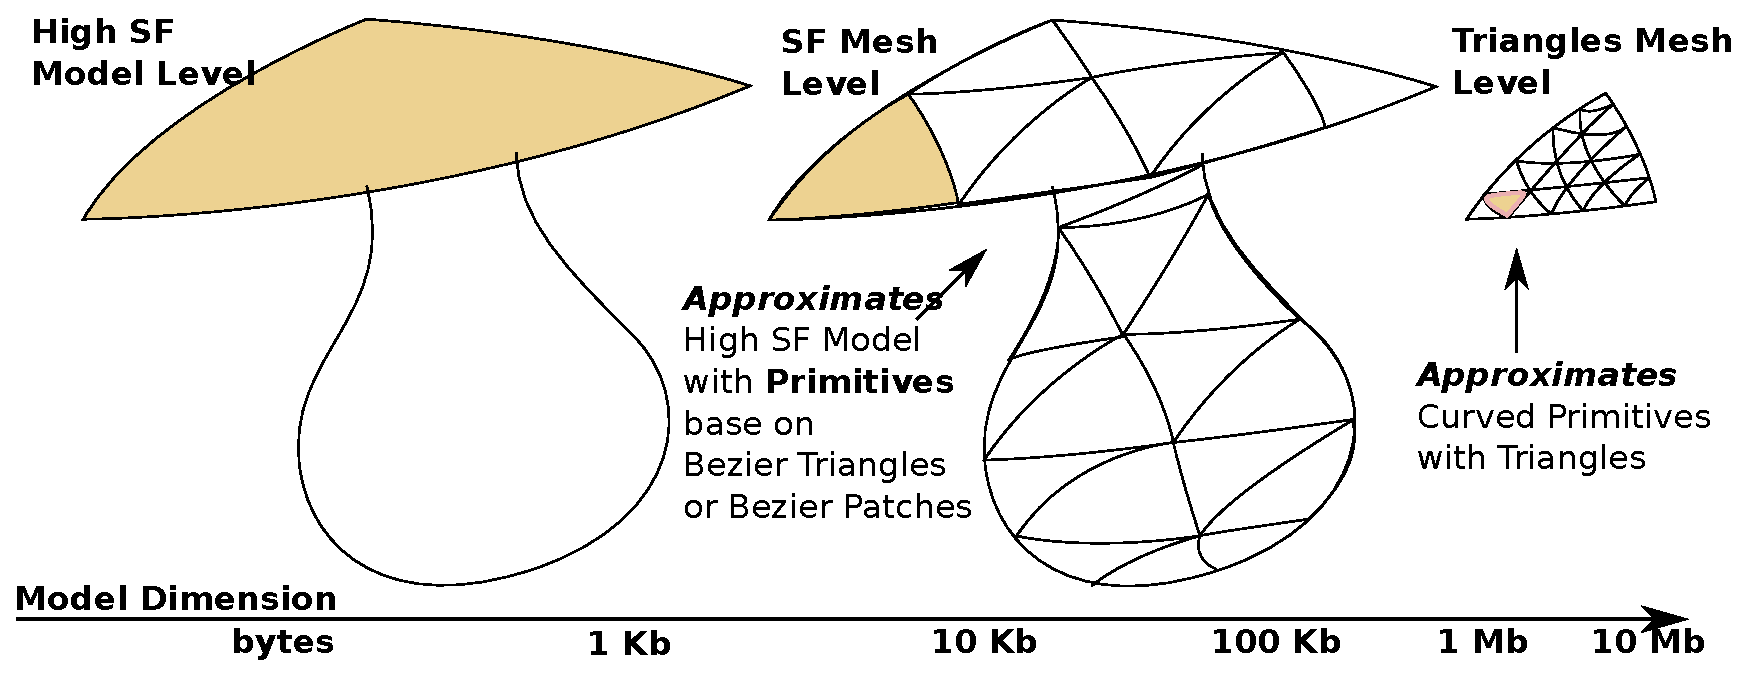
\includegraphics[width=\textwidth]{Immagini/hierarchicalmodeling}
\caption{Grafico della modellizzazione gerarchica del framework.\label{f:hierarchicalmodeling}} 
\end{center} 
\end{figure}

In figura \ref{f:hierarchicalmodeling} possiamo vedere come questa gerarchizzazione sia strutturata a due vie: sulla sinistra vediamo l'oggetto modellizzato ad alto livello, i file sf del framework contengono i dati riferiti a questo livello di astrazione che risultano molto compatti (dai pochi kbyte a qualche decina), ma comunque ricchi di informazioni.
La prima decompressione delle informazioni consiste nel tassellare\footnote{La tassellazione \`e un processo attraverso cui una superficie viene suddivisa in poligoni non sovrapposti.\cite{book:realtimerendering}} il modello parametrico con primitive di alto livello adatte allo scopo, in figura sono citati i triangoli di Bezier e le patch di Bezier. I dati estratti da questa prima fase possono raggiungere le centinaia di \ac{kB}. La seconda fase consiste in una ulteriore tassellazione delle primitive di alto livello in triangoli veri e propri che approssimano le superfici curve delle precedenti primitive e che possono essere usati direttamente della \ac{GPU} per effettuare il rendering. Questa operazione genera quantit\`a di dati la cui dimensione pu\`o essere anche di decine di \ac{MB}, ma essendo eseguita direttamente all'interno della memoria grafica il trasferimento ne risulta alleggerito. Il valore aggiunto di questa gerarchizzazione \`e che sfruttando su pi\`u livelli i processi di tassellazione ha intrinsecamente al suo interno un modo per scalare il livello di dettaglio modificando la granularit\`a della tassellazione stessa, evitando la duplicazione dei dati.

\subsection{Considerazioni finali sul framework}
La naturale premessa, essenziale per supportare le valutazioni espresse nei precedenti paragrafi, corrisponde alla necessit\`a da parte del framework di utilizzare un set di strutture geometrie intelligenti adatte allo scopo. Questo set deve soddisfare una serie di requisiti fondamentali senza i quali il framework incontrerebbe serie problematiche di applicabilit\`a e usabilit\`a, questi requisiti sono:
\begin{itemize}
	\item  la \textbf{completezza}, ovvero deve essere in grado di rappresentare ogni tipo di superficie del mondo reale;
	\item  la \textbf{semplicit\`a}, in quanto un set troppo complesso e articolato renderebbe il processo di selezione delle geometrie problematico;
	\item  la \textbf{flessibilit\`a}, nel senso che le geometrie devono essere in grado di scalare efficacemente in qualit\`a per venire incontro alle capacit\`a di apparecchiature differenti.
\end{itemize}

Questo \`e uno degli aspetti di ricerca e sperimentazione pi\`u interessanti del framework che, sebbene sia gi\`a sufficientemente maturo, \`e attualmente oggetto di ulteriore sviluppo.

\section{Struttura dello Shadow Framework 2.0}
\label{sec:sfstructure}
\begin{figure}
\begin{center}
\includegraphics[width=10cm]{Immagini/sfstructure}
\caption{Struttura dei moduli del framework.\label{f:sfstructure}} 
\end{center} 
\end{figure}
Il framework \`e strutturato in moduli gerarchici e la figura \ref{f:sfstructure} ne illustra i livelli e le loro dipendenze. Il livello pi\`u basso \`e quello denominato \textbf{system} e contiene al suo interno le astrazioni base sfruttate da tutti gli altri moduli. Ad un livello superiore troviamo il modulo \textbf{data} che si occupa di tutti gli aspetti riguardanti la gestione dati all'interno del framework. Per raggiungere gli obbiettivi prefissati il progetto di tesi \`e incentrato sull'estensione delle funzionalit\`a di questo livello e il capitolo \ref{ch:gestionedati} offre un approfondimento su meccanismi e le astrazioni su cui \`e fondato. Il livello \textbf{graphics} offre un'astrazione su di una pipeline di rendering ideale di cui possiamo osservare una rappresentazione in figura \ref{f:sfpipeline}. Dato che non esiste una implementazione diretta di questa pipeline, il framework la realizza configurando una pipeline programmabile attraverso l'\ac{API} OpenGL a cui si interfaccia tramite il modulo \textbf{graphics OpenGL}.
\begin{figure}
\begin{center}
\includegraphics[width=\textwidth]{Immagini/Pipeline}
\caption{Rappresentazione della pipeline ideale implementata dal framework.\label{f:sfpipeline}} 
\end{center} 
\end{figure}
Al di sopra del modulo graphics vi \`e \textbf{rendering}, che contiene il rendering engine vero e proprio che basa il suo funzionamento sulle caratteristiche della pipeline astratta del livello inferiore.
Il livello \textbf{rendering data} definisce infine la struttura dei dati grafici, questa struttura dipende dai livelli inferiori perch\`e deve tenere conto del modulo data per quanto concerne il reperimento dei dati, e del modulo rendering per i meccanismi di costruzione dei dati.

Le applicazioni costruite basandosi sul framework non hanno necessità di operare direttamente sulle \ac{API} grafiche a basso livello, ma possono essere strutturate per lavorare sulle astrazioni di alto livello offerte dal framework.

La versione del framework di riferimento, nonch\`e quella oggetto di sviluppo in questo progetto di tesi, \`e quella realizzata in linguaggio Java e disponibile tramite la fonte indicata al paragrafo \ref{sub:sfsource}. 
Per questa versione il modulo \textbf{graphics OpenGL} non si interfaccia direttamente con le \ac{API} OpenGL, ma sfrutta a tal scopo la libreria del progetto JOGL\footnote{Per informazioni sulla libreria JOGL fare riferimento al paragrafo \ref{sub:jogl}.}.

%!TEX root = ../tesi.tex

\chapter{Gestione dei dati nello Shadow Framework 2.0}
\label{ch:gestionedati}

% TODO: ampliare l'introduzione
La gestione dei dati \`e un compito molto importante all'interno del framework. Attraverso l'utilizzo di un layer di gestione dati astratto, ogni mudulo del framework pu\`o essere salvato e caricato da file o trasferito attraverso un qualsiasi flusso di dati.
In questo capitolo viene presentata l'astrazione utilizzata dallo Shadow Framework nella gestione dei dati, le funzionalit\`a messe a disposizione ed i principali package e moduli coinvolti.

\begin{figure}
\begin{center}
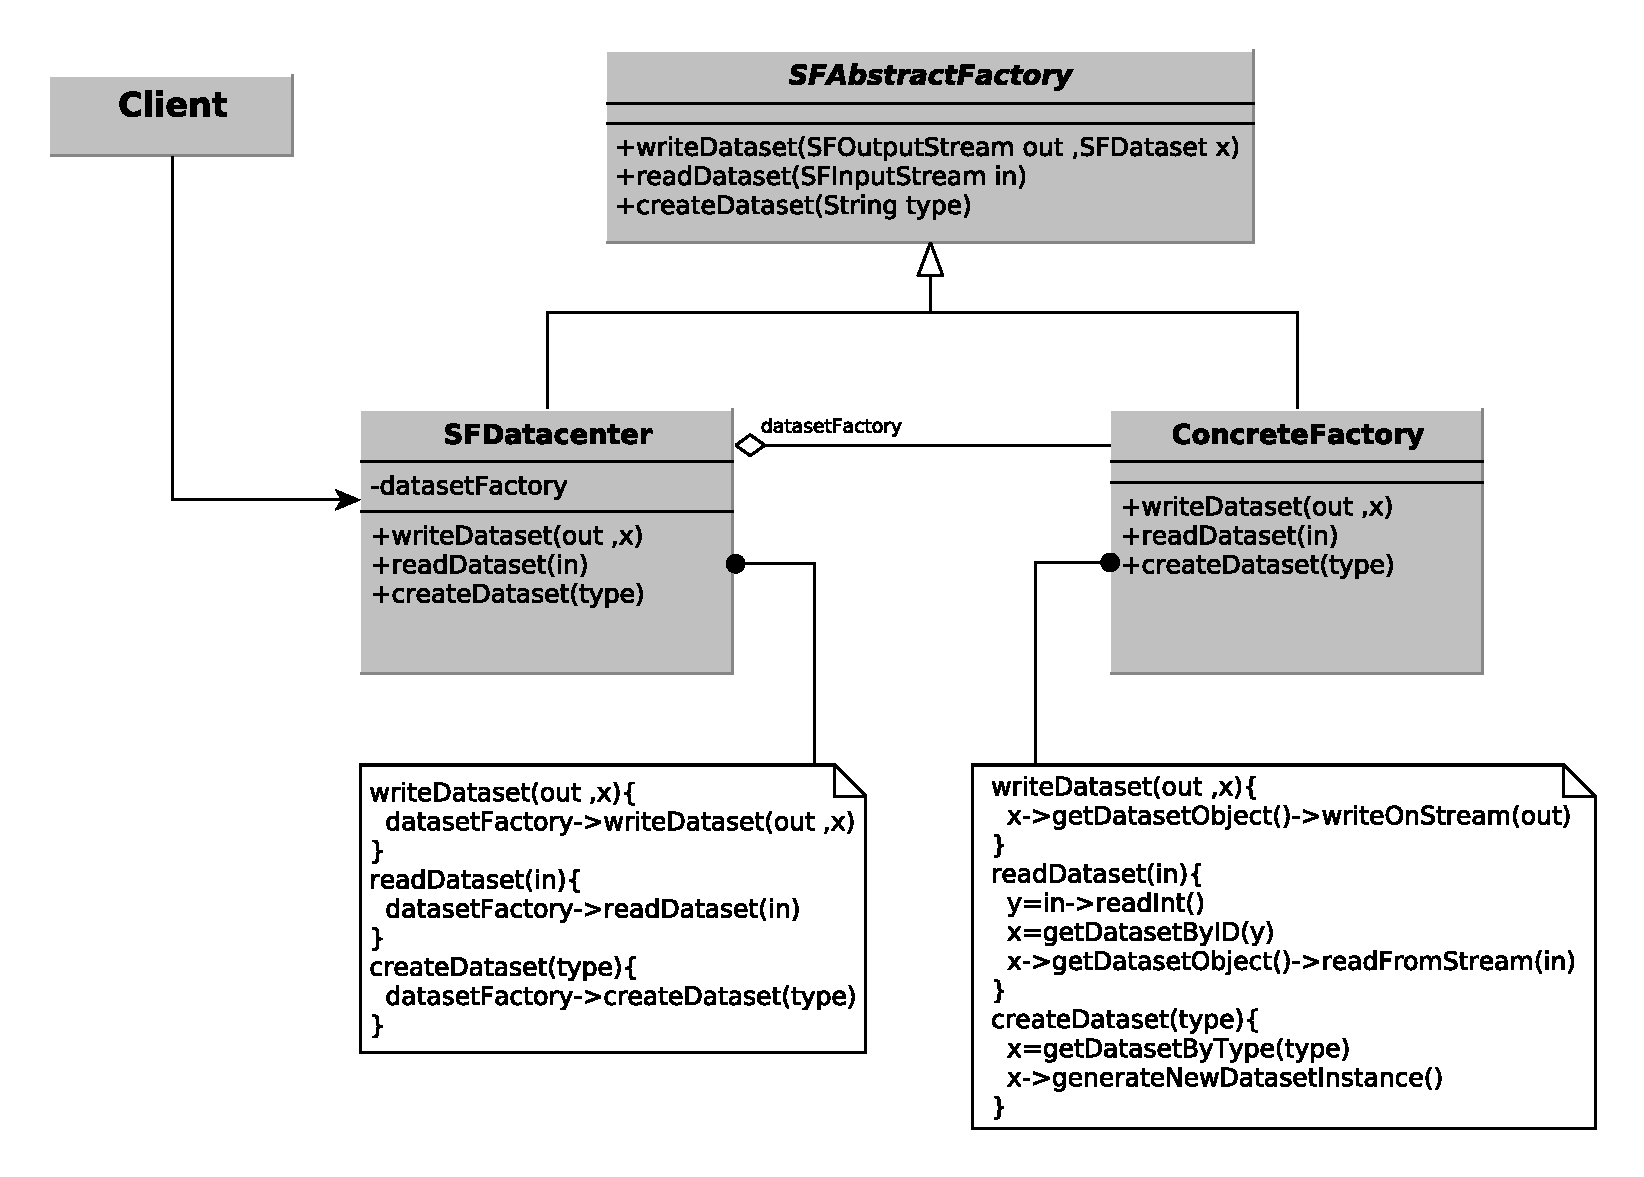
\includegraphics[width=\textwidth]{Immagini/DataCenterfactory}
\caption[Bridge composto da SFDataCenter e SFAbstractFactory]{Diagramma del Bridge composto da SFDataCenter e da un'istanza concreta di SFAbstractFactory.\label{f:datacenterfactory}} 
\end{center} 
\end{figure}

\section{L'astrazione della gestione dati}
\label{sec:astrazione}
All'interno di un'applicazione \ac{SF} l'unit\`a base di dati pu\`o essere identificata con quello che viene definito SFDataset e di cui si pu\`o trovare una descrizione pi\`u dettagliata al paragrafo \ref{sub:sfdataset}. Con Dataset si identifica quasi ogni tipo di dato, sia grafico che non, utilizzato all'interno del framework.
La gestione dei dataset viene effettuata mediante un meccanismo centralizzato: ogni applicazione in esecuzione possiede un'istanza di SFDataCenter, questa classe \`e un oggetto \textit{Singleton} che realizza un \textit{Bridge}
tra l'astrazione di reperimento dati e la sua implementazione concreta\footnote{Con \textit{Singleton} e \textit{Bridge} si intendono i design pattern omonimi descritti pi\`u in dettaglio nell'appendice \ref{a:designpatterns}}.
Ogni componente pu\`o accedere al DataCenter per richiedere operazioni sui Dataset di interesse, operazioni che possono essere la lettura o la scrittura da uno stream specifico, la richiesta di una particolare istanza di un Dataset, identificata per nome, o la richiesta di una nuova istanza di Dataset, identificata per tipo.
L'oggetto Singleton espone queste funzionalit\`a traducendole internamente con chiamate ad una factory concreta\footnote{Si fa riferimento al pattern di programmazione \textit{Abstract Factory} descritto nella sezione \ref{sub:abstractfactory}}
di Dataset e ad una istanza dell'interfaccia SFIDataCenter, creando un'astrazione su come i Dataset siano effettivamente costruiti e reperiti esattamente come mostrato nelle immagini \ref{f:datacenterfactory} e \ref{f:datacenterimplementation}
La factory concreta deve essere un'implementazione dell'interfaccia SFAbstractDatasetFactory in grado di istanziare, leggere o scrivere ogni tipo di Dataset utilizzato dall'applicazione.
L'istanza dell'interfaccia SFIDataCenter tiene traccia dei Dataset istanziati con nome, restituendone un riferimento a chi ne fa richiesta attraverso la chiamata a funzioni di callback.

\begin{figure}
\begin{center}
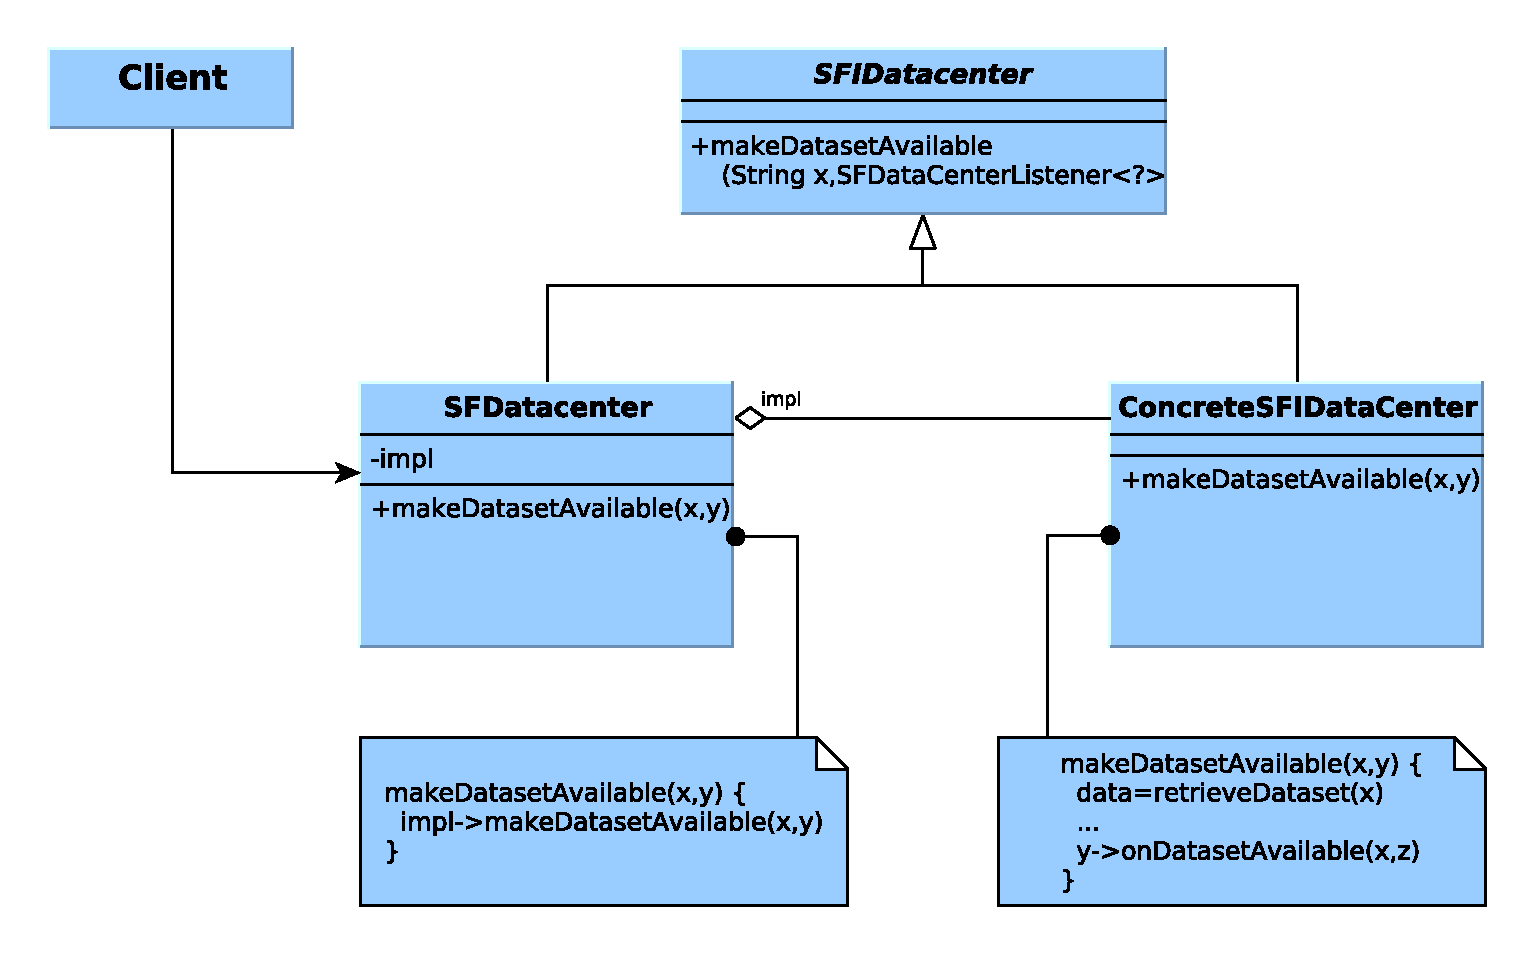
\includegraphics[width=\textwidth]{Immagini/DataCenter}
\caption[Bridge composto da SFDataCenter e SFIDataCenter]{Diagramma del Bridge composto da SFDataCenter e da un'istanza concreta di SFIDataCenter.\label{f:datacenterimplementation}} 
\end{center} 
\end{figure}
% TODO: aggiungere immagine


\section{Il package \texttt{shadow.system.data}}
\label{sec:shadow_system_data}
Questo package contiene una serie di classi ed interfacce su cui si basa l'astrazione dei dati del framework.

\subsection{SFInputputStream e SFOutputStream}
\label{sub:sfinoutstream}
Queste interfacce definiscono le operazioni necessarie che uno stream di input o di output deve implementare affinch\'e sia possibile leggere o scrivere su di esso dei DataObject e insieme costituiscono un elemento molto importante per l'estendibilit\`a del framework sui dati. Su di esse si basa infatti l'astrazione che i dati utilizzano per completare le operazioni di lettura e scrittura. Utilizzando la medesima interfaccia di astrazione \`e possibile far comunicare tra loro anche implementazioni diverse del framework.

\subsection{SFDataObject}
\label{sub:sfdataobject}
Uno dei moduli principali del package \`e \texttt{SFDataObject}, che rappresenta un'interfaccia con funzionalit\`a di base comuni ad ogni oggetto che contiene dati. 
Ogni oggetto di questo tipo pu\`o perci\`o:
\begin{itemize}
	\item essere scritto su di un \texttt{SFOutputStream};
	\item essere letto da un \texttt{SFInputStream};
	\item essere clonato;
\end{itemize}
I DataObject si basano sul \textit{Composite Pattern}\ref{sub:composite}: possono essere semplici o contenere un insieme di oggetti figli, il fatto che sia gli oggetti complessi che gli oggetti semplici condividano la stessa interfaccia permette di trattare gli oggetti in modo uniforme. Un oggetto contenitore dovr\`a semplicemente richiamare lo stesso metodo di interfaccia per tutti gli oggetti figli i quali, se oggetti semplici, hanno la responsabilit\`a di implementare l'algoritmo per leggere o scrivere se stessi da uno stream.

Tutti i componenti SF utilizzano dei DataObject per incapsulare i dati in modo che questi ultimi possano essere letti e scritti utilizzando stream appropriati.

\begin{figure}
\begin{center}
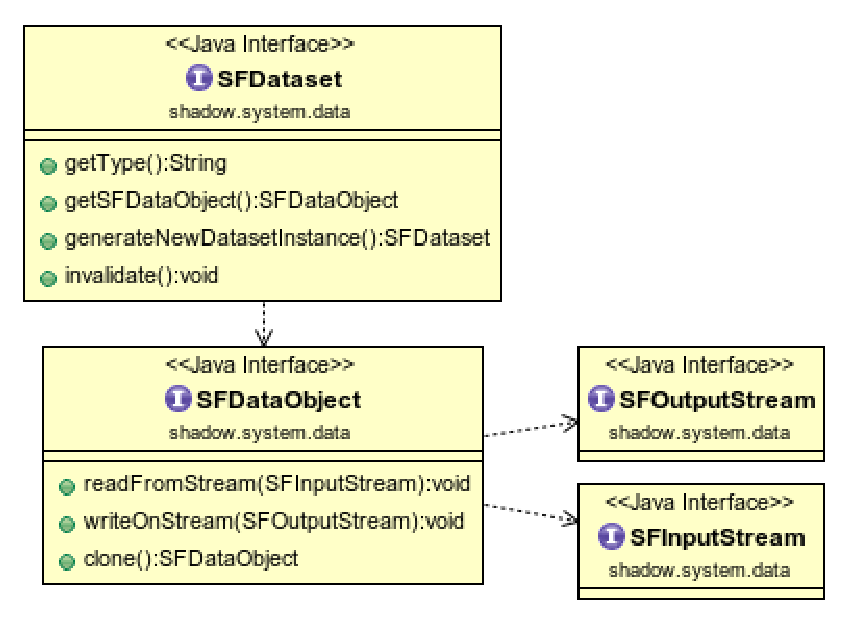
\includegraphics[width=11cm]{Immagini/relazione-dataset-dataobject-stream}
\caption{Diagramma della relazione tra le classi SFDataset, SFDataObject, SFInputStream e SFOutputStream.\label{f:dataset-dataobj-stream}} 
\end{center} 
\end{figure}

\subsection{SFDataset}
\label{sub:sfdataset}
Un altro modulo importante per la gestione dei dati \`e \texttt{SFDataset}. Un Dataset \`e un oggetto che contiene un DataObject e informazioni sul proprio tipo, rappresentato tramite una stringa.
Da come si pu\`o intuire dalla figura \ref{f:dataset-dataobj-stream} il DataObject viene sfruttato dal Dataset per incapsulare i suoi dati interni ed incorporarne le funzionalit\`a di lettura e scrittura.
L'interfaccia SFDataset definisce un'interfaccia per oggetti di questo tipo, la quale consente di accedere al nome del tipo specifico, al DataObject contenuto e di creare una nuova istanza delle stesso tipo.
A loro volta i Dataset possono essere incapsulati in un DataObject usando un oggetto \texttt{SFDatasetObject}.

\subsection{SFAbstractDatasetFactory}
\label{sub:sfabstractdatasetfactory}
Questa interfaccia definisce le operazioni base richieste ad una DatasetFactory, queste operazioni consistono in:
\begin{itemize}
	\item lettura/scrittura di un Dataset da uno stream
	\item la creazione di una nuova istanza di un Dataset specificato per tipo
\end{itemize}

\subsection{SFIDataCenter}
\label{sub:sfidatacenter}
L'interfaccia \texttt{SFIDataCenter} fornisce l'astrazione di una Mappa di Dataset identificati attraverso il proprio nome, attraverso di essa possiamo chiedere di recuperare un Dataset ad un oggetto che la implementa.
Quest'oggetto non deve restituire direttamente il Dataset recuperato, ma deve farlo attraverso un meccanismo di callback ad una implementazione dell'interfaccia \texttt{SFDataCenterListener} passata come parametro, nel momento in cui il dato \`e disponibile.

\begin{figure}
\begin{center}
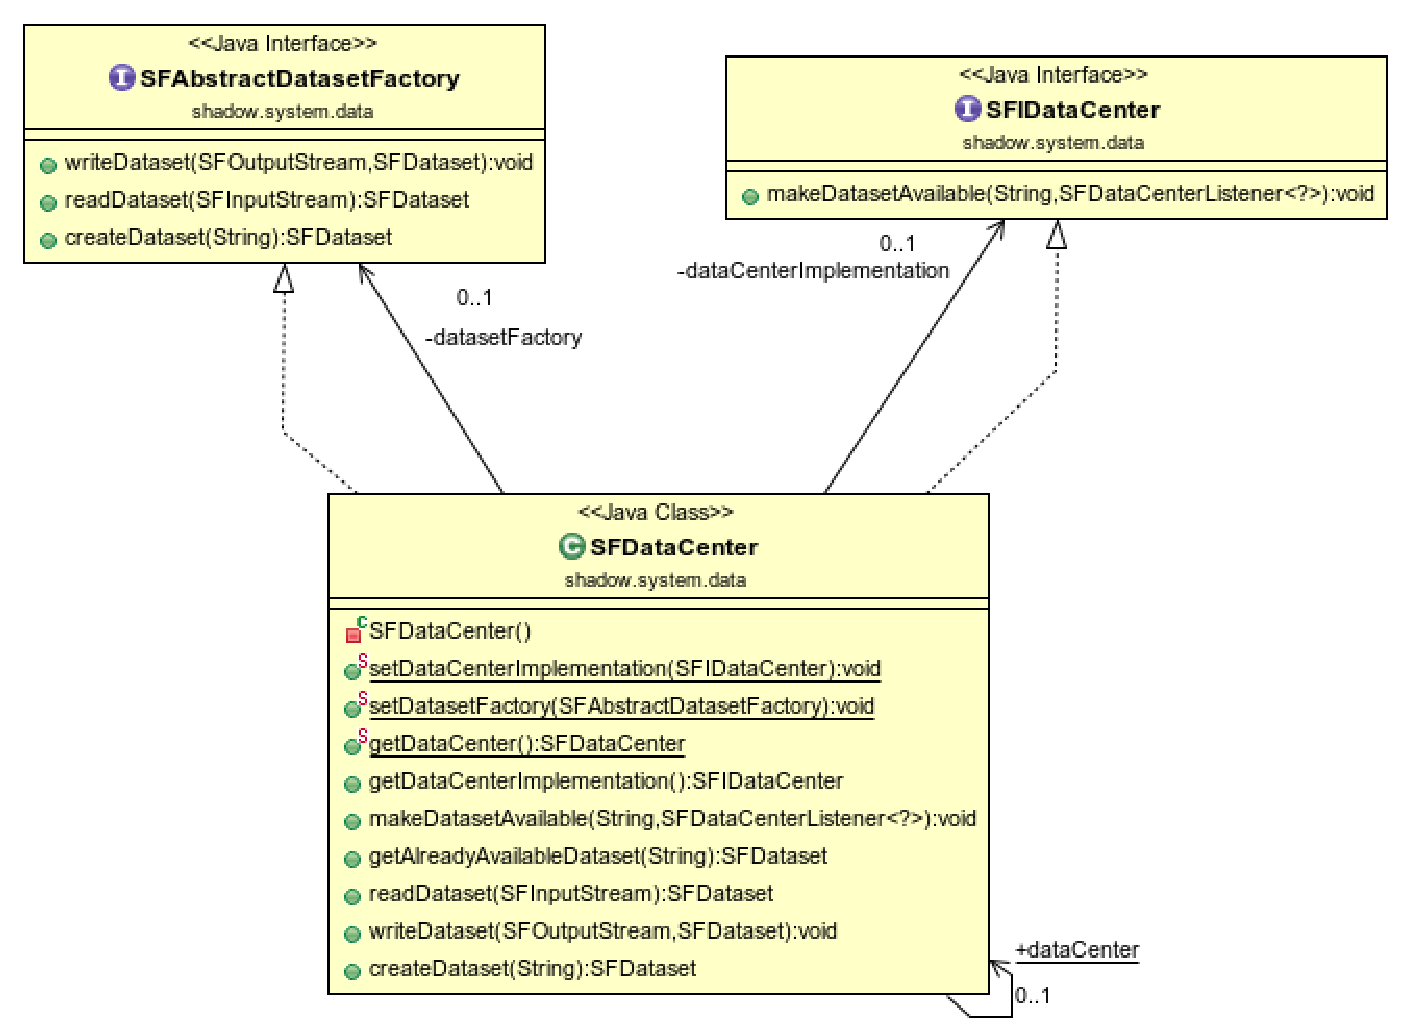
\includegraphics[width=\textwidth]{Immagini/DataCenterBridge}
\caption{In questo diagramma viene mostrata la relazione tra le classi SFDataCenter, SFIDataCenter e SFAbstractDatasetFactory. Da notare che SFDataCenter \`e una classe Singleton in quanto contiene una istanza statica di se stessa (l'istanza dataCenter sottolineata) e possiede un costruttore privato (evidenziato in rosso). Inoltre, in riferimento alla sezione \ref{sub:bridge}, si pu\`o notare come SFDataCenter realizzi un Bridge sia con SFIDataCenter che con SFAbstractDatasetFactory \label{f:datacenterbridge}} 
\end{center} 
\end{figure}

\subsection{SFDataCenterListener}
\label{sub:sfdatacenterlistener}
Questa interfaccia definisce la callback che un componente deve implementare per effettuare una richiesta al DataCenter.
Questa callback viene richiamata quando il Dataset richiesto \`e pronto.

\subsection{SFDataCenter}
\label{sub:sfdatacenter} 
% TODO: evitare di ripetere quanto detto in sec:astrazione
Il \textbf{DataCenter} \`e il nodo fondamentale della gestione dei dati all'interno del framework. 

\'E un oggetto \textit{Singleton} (\ref{sub:singleton}) a cui le applicazioni accedono per richiedere i Dataset di cui hanno bisogno. Questa classe utilizza anche il pattern \textit{Bridge} (\ref{sub:bridge}) per fornendo un'astrazione su come i dati sono effettivamente reperiti.

Per poter funzionare, al DataCenter deve essere fornita un'implementazione per:
\begin{itemize}
	\item \texttt{SFAbstractDatasetFactory}
	\item \texttt{SFIDataCenter}
\end{itemize}

Come precedentemente esposto, l'implementazione di \texttt{SFAbstractDatasetFactory} deve essere essere una factory in grado di generare istanze di tutti i tipi di Dataset necessari all'applicazione.

Questo tipo di astrazione permette di separare la logica di utilizzo del Dataset da quella di come esso viene reperito, consentendo ad una applicazione di usare dati locali o dati di rete semplicemente cambiando l'implementazione di \texttt{SFIDataCenter}.

\subsection{SFObjectsLibrary}
\label{sub:sfobjectslibrary}
\'E usata per memorizzare un set di Dataset ed al suo interno ogni elemento \`e identificato tramite un nome univoco.
Un \texttt{SFObjectsLibrary} \`e a sua volta un Dataset, cos{\`\i} che un ObjectsLibrary possa essere contenuta in altre ObjectsLibrary.
\'E possibile, ad esempio, utilizzare una ObjectLibrary all'interno di implementazione di \texttt{SFIDataCenter} per creare una mappa di Dataset necessari al funzionamento di un'applicazione.

\section{Classi di utilit\`a per il layer dati}

\subsection{SFLibraryreference}
\label{sub:sflibraryreference}
Un LibraryReference \`e un DataObject che pu\`o essere usato da qualsiasi componente per avere un riferimento ad un Dataset memorizzato in una libreria. Viene utilizzato all'interno di DataObject o di Dataset per non avere istanze doppie dello stesso dato.


\subsection{SFGenericDatasetFactory}
\label{sub:sfgenericdatasetfactory}
Questa classe di utilit\`a consiste in una implementazione concreta di default dell'interfaccia \texttt{SFAbstractDatasetFactory}.
Per consentire il riutilizzo del codice \`e stata resa configurabile: l'aggiunta di un metodo addSFDataset() consente di generare, in un oggetto GenericDatasetFactory, un elenco di Dataset istanziabili.
Quando verranno chiamati i metodi dell'interfaccia SFAbstractDatasetFactory sull' oggetto GenericDatasetFactory diviene sufficiente richiamare il metodo opportuno del Dataset del tipo richiesto o del DataObject in esso contenuto.
%!TEX root = ../tesi.tex

\chapter{Il Progetto SF-Remote-Connection}
\label{ch:sfremoteconnection}

Vengono ora presentati i moduli software realizzati nel corso dello sviluppo del progetto di tesi.
Per meglio comprendere gli aspetti di sviluppo legati al progetto \`e importante tener conto degli obbiettivi di progetto esposti al paragrafo \ref{sec:obbiettivo} e della descrizione dei meccanismi di gestione dati interni del framework, descritti nel capitolo \ref{ch:gestionedati}.

Nella sezione \ref{sec:moduli} del capitolo viene fornita innanzitutto una suddivisione e una descrizione dei moduli, nella sezione \ref{sec:dataset_sost} viene descritto il meccanismo dei Dataset sostitutivi
e nella \ref{sec:rete} l'infrastruttura di ret e il protocollo di comunicazione.
Infine \`e presente una panoramica sui package java e le principali classi di ognuno di essi nella sezione \ref{sec:sfrc_packages}.

\`E giusto sottolineare che l'obbiettivo principale \`e stato la produzione di librerie e tool per lo sviluppo di applicazioni, focalizzandosi sull'estendibilit\`a e il riutilizzo del codice. Non a caso sono infatti presenti alcuni riferimenti di appendice ad alcuni design pattern particolarmente significativi nella produzione di questo tipo di softwaree e che sono utilizzati sia dal framework che dai moduli stessi.

Per il processo di sviluppo \`e stata di fondamentale importanza la produzione parallela di una serie di test, presentati nel capitolo \ref{ch:testerisultati}. Infatti la progettazione e la realizzazione dei moduli e dei meccanismi presentati in questo capitolo non \`e stata svolta in maniera distinta, ma si \`e trattato di un processo iterativo in cui i test hanno svolto pi\`u di una volta un ruolo di guida nel refactoring del codice.

Si rimanda all'appendice \ref{a:notesoftware} per informazioni sul codice sorgente relativo al progetto e per informazioni sulle versioni delle librerie utilizzate.

% TODO: cambiare titolo?
\section{Moduli} 
\label{sec:moduli}
La libreria di classi realizzata pu\`o essere suddivisa in quattro macro-moduli suddivisi in base alle finalit\`a e alle funzionalit\`a.
Di seguito viene data una descrizione degli stessi in questo ordine:
\begin{enumerate}
	\item \textbf{Base Communication}
	\item \textbf{RemoteDataCenter Tool}
	\item \textbf{Client}
	\item \textbf{Server}
\end{enumerate}

% TODO: 
%	inserire un'immagine di come i moduli funzionino su vari livelli
%	verificare i nomi e le appartenenze dei package

\subsection{Base Communication}
\label{sub:basecommodule}
Questo modulo riunisce le classi che consentono la creazione e la gestione di connessioni TCP/IP tra applicazioni client/server. Ne fa parte anche la classe di utilit\`a \texttt{GenericCommunicator} che oltre a consentire la gestione della connessione assegnatagli la utilizza per fornire funzionalit\`a di lettura e scrittura di messaggi testuali attraverso il canale aperto.

Il modulo \`e composto dai package \texttt{sfrc.base.communication} e \\\texttt{sfrc.base.communication.sfutil}.

\subsection{RemoteDataCenter Tool}
\label{sub:remotedatacentertoolmodule}

\begin{figure}[t]
\begin{center}
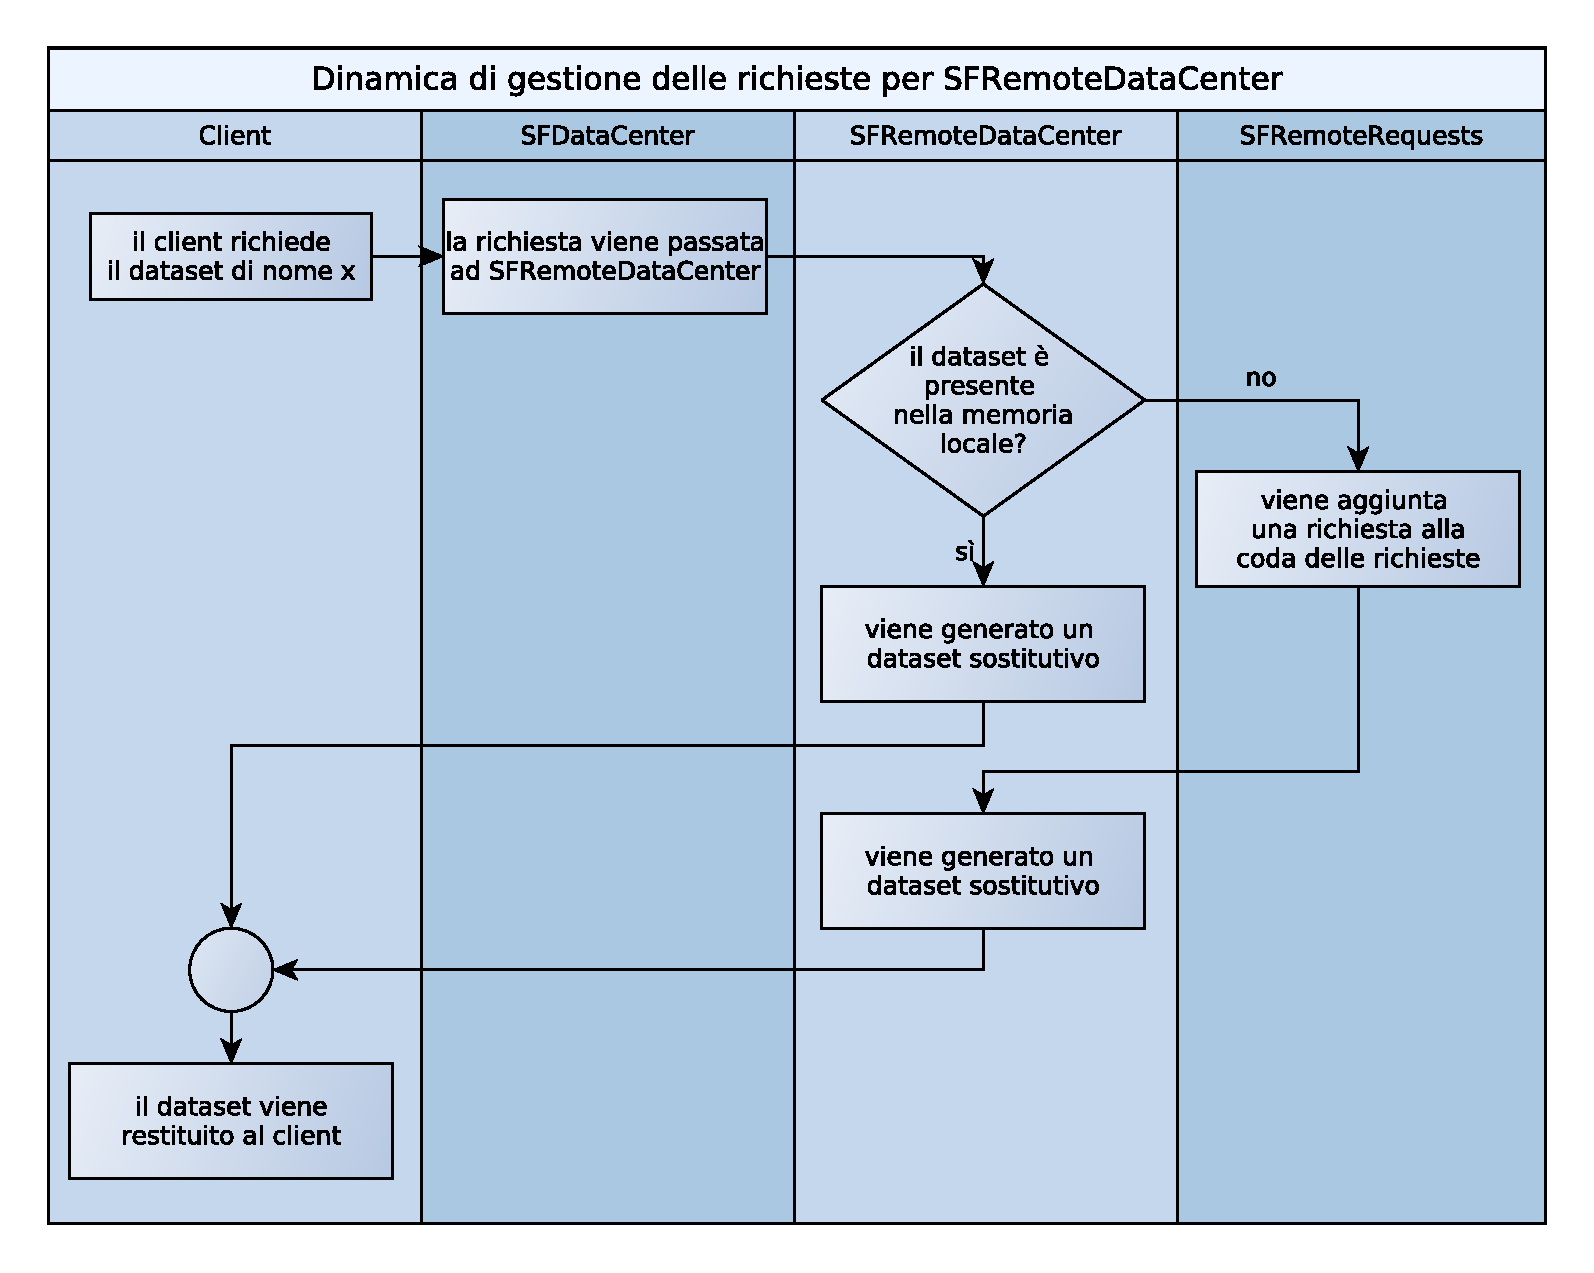
\includegraphics[width=\textwidth]{Immagini/DinamicaSFRemoteDataCenter}
\caption{Lo schema mostra la sequenza di eventi dovuti ad una richiesta a SFDataCenter che utilizza un SFRemoteDataCenter come implementazione interna.\label{f:dinamicasfremotedatacenter}} 
\end{center} 
\end{figure}

Questo modulo raggruppa una serie di classi pensate per essere una estensione del framework e per essere utilizzate principalmente all'interno di una applicazione client.
La sua funzione principale consiste nel fornire uno strato di comunicazione tra l'astrazione del reperimento dati fornita dal framework e il meccanismo di effettivo reperimento dei dati.

La classe chiave del modulo \`e \texttt{SFRemoteDataCenter}: questa \`e una classe di implementazione utilizzabile nel \textit{Bridge} realizzato da \texttt{SFDataCenter}\footnote{Per la classe \texttt{SFDataCenter} si rimanda al paragrafo \ref{sub:sfdatacenter} mentre per il pattern \textit{Bridge} al paragrafo \ref{sub:bridge}.}.
Dallo schema in figura \ref{f:dinamicasfremotedatacenter} osserviamo che le richieste di Dataset effettuate al DataCenter vengono passate a questa classe che le esamina verificando che il dato richiesto sia presente nella libreria dell'applicazione. Se il Dataset non \`e presente viene generata una richiesta e aggiunta ad un buffer di richieste di nome SFRemoteRequests, successivamente al richiedente \`e restituito un Dataset sostitutivo temporaneo scelto opportunamente. Il buffer, che supporta la sincronizzazione, pu\`o contemporaneamente essere utilizzato da un modulo esterno in grado di effettuare l'effettivo reperimento dei dati.
Il meccanismo dei Dataset sostitutivi viene descritto esaustivamente nella sezione \ref{sec:dataset_sost}.

% TODO: decidere se i 2 package aggiuntivi andrebbero inseriti nel modulo
Il modulo \`e composto dai package \texttt{shadow.system.data.remote.wip}, \texttt{shadow.system.data.object.wip} e \texttt{shadow.renderer.viewer.wip}.

\subsection{Client}
\label{sub:clientmodule}
Questo modulo raggruppa delle componenti generiche che possono essere utilizzate all'interno di una qualsiasi applicazione client e che servono ad implementare l'effettivo reperimento dei dati. 
Esso si pone al di sotto del modulo \textbf{RemoteDataCenter Tool} ed utilizza il modulo \textbf{Base Communication} per la gestione del canale di comunicazione e la sua implementazione \`e pensata per il multi-threading.
Il meccanismo messo a disposizione \`e mostrato nella figura \ref{f:dinamicaclient}, in esso un thread \texttt{RemoteDataCenterRequestsCreationTask} viene risvegliato periodicamente e controlla che non vi siano richieste pendenti nel buffer delle richieste. Se il buffer non \`e vuoto viene allora allocano un nuovo thread di tipo \texttt{RemoteDataCenterRequestTask} e mentre il precedente viene nuovamente sospeso questo effettua le richieste al server. Quando il secondo thread termina la comunicazione chiede al buffer di generare un update a tutti i client che avevano richiesto i dati reperiti e successivamente si chiude.


\begin{figure}
\begin{center}
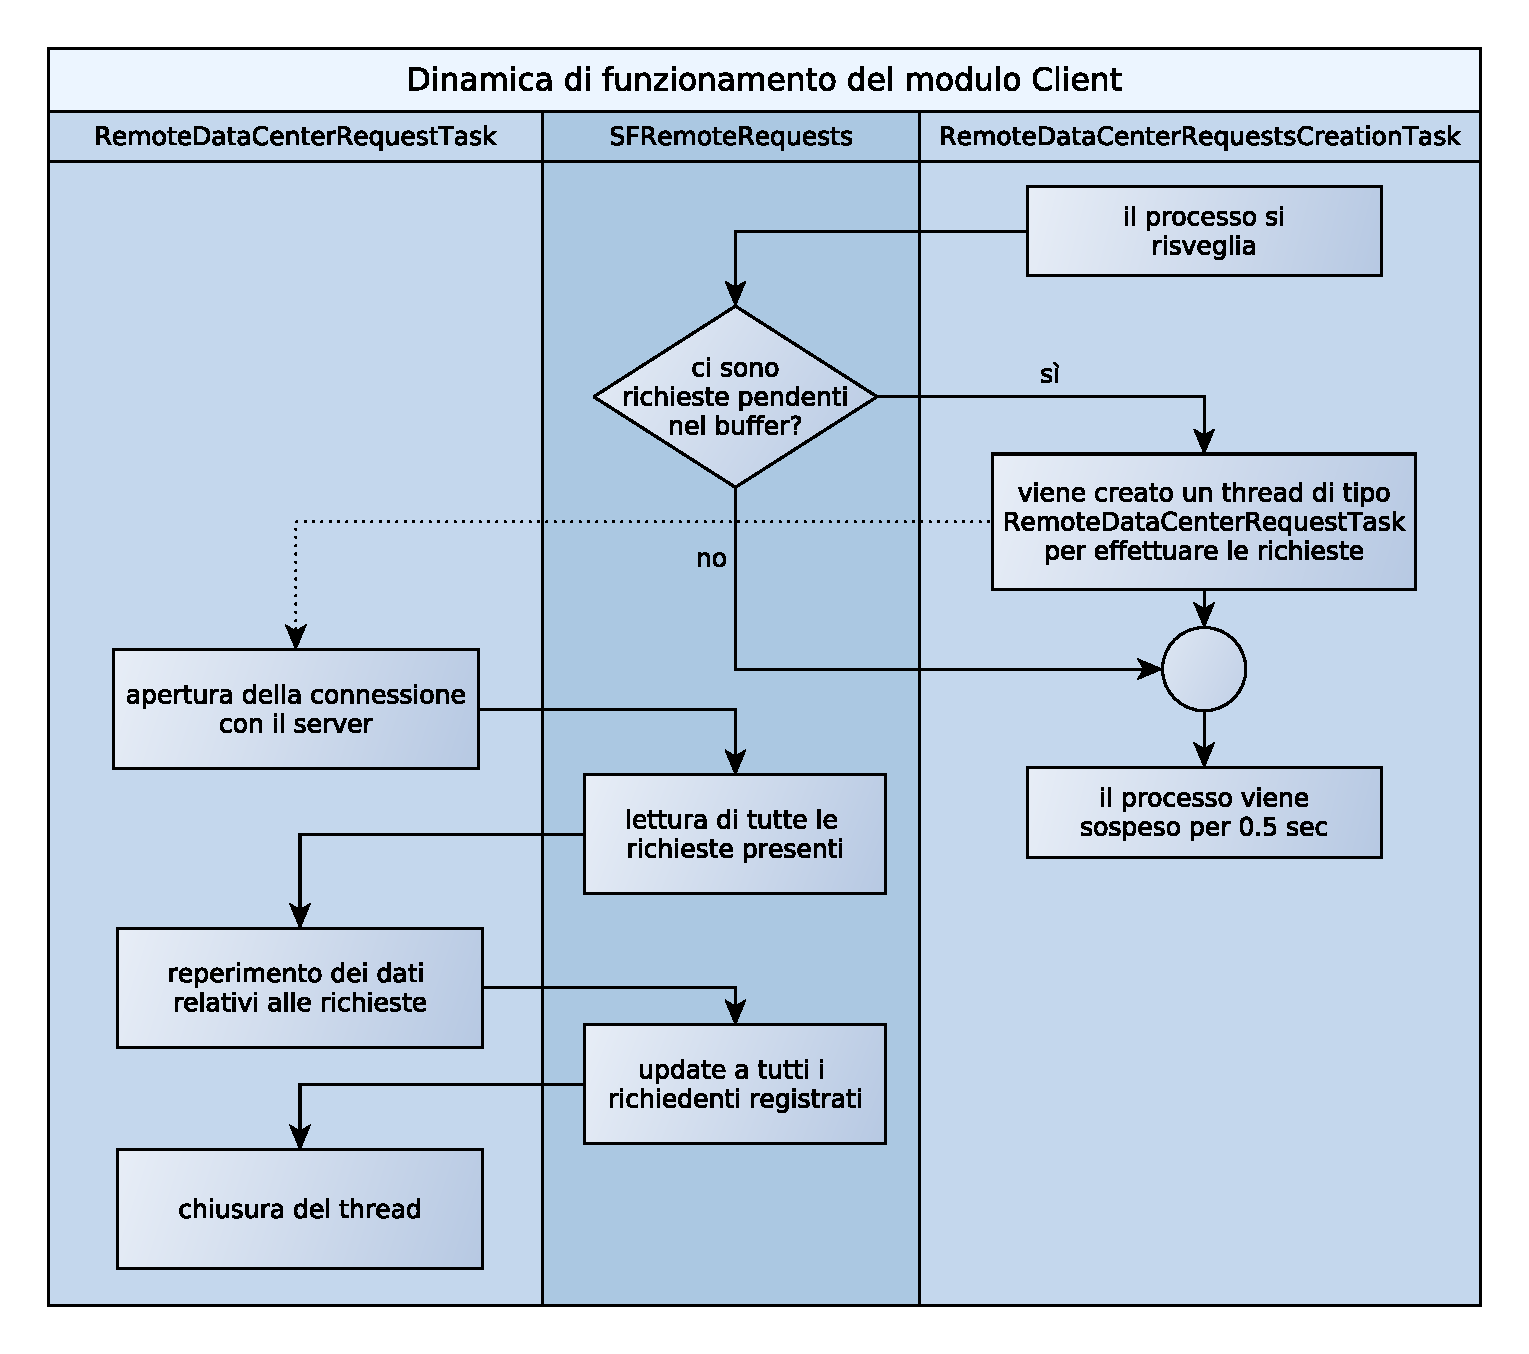
\includegraphics[width=\textwidth]{Immagini/DinamicaClient}
\caption{Dinamica del modulo client. Nello schema viene messa in evidenza la sostanziale indipendenza dei thread \texttt{RemoteDataCenterRequestsCreationTask} e \texttt{RemoteDataCenterRequestTask}, infatti a parte il fatto che i thread del secondo tipo sono creati dal primo non vi sono comunicazioni dirette tra i due.\label{f:dinamicaclient}} 
\end{center} 
\end{figure}


Il package che compone questo modulo \`e \texttt{sfrc.application.client}.

\subsection{Server}
\label{sub:servermodule}
Similmente al modulo per le componenti client, in questo vengono raggruppate delle componenti generiche utili alla realizzazione di una applicazione server. Queste componenti si pongono da tramite tra l'applicazione e il modulo di \textbf{Base Communication} tramite cui realizzano l'effetivo trasferimento dei Dataset verso il client connesso.
Anche in questo caso l'implementazione \`e pensata per il funzionamento multi-thread in parallelo con l'applicazione principale che pu\`o cos{\`\i} gestire pi\`u client connessi contemporaneamente ed eseguire altre operazioni.
Vengono fornite infine anche delle interfacce utili per effettuare l'inizializzazione dei dati e per configurare il protocollo di comunicazione.

Il modulo \`e composto dal package \texttt{sfrc.application.server}

\section{Dataset sostitutivi}
\label{sec:dataset_sost}
Per evitare che, in seguito alla richiesta di un Dataset non presente nella libreria locale di un'applicazione, i moduli richiedenti rimanessero in attesa dei dati bloccando di fatto l'esecuzione, \`e stato deciso di realizzare un meccanismo di sostituzione dei Dataset con successivo update delle richieste.
Successivamente ad una richiesta il RemoteDataCenter restituisce, attraverso la callback del richiedente, un Dataset sostitutivo temporaneo di tipo compatibile a quello richiesto.
Contemporaneamente viene generata una richiesta remota che attende di essere evasa. Quando i dati effettivi arrivano dalla rete viene eseguito un update del dato richiamando nuovamente la callback del richiedente.
Dato che pi\`u moduli dell'applicazione potrebbero fare richiesta dello stesso Dataset, tutte le callback dei richiedenti vengono memorizzate e, al momento dell'update, richiamate in successione.
% TODO: decidere se parlare dell'Updater
Per permettere il funzionamento di questo automatismo si \`e resa necessaria la realizzazione di un nuovo tipo di Dataset, l'SFDatasetReplacement, e di una libreria di Dataset sostitutivi.

Utilizzato all'interno di una ObjectsLibrary un DatasetReplacement permette di realizzare una lista di sostituzione che associa il nome di un Dataset "Alfa" richiesto, a quello di un Dataset sostitutivo di default "Beta" e ad un timestamp.
L'associazione tra nomi viene usata per una ricerca diretta del dato sostitutivo da utilizzare, mentre il timestamp \`e stato introdotto per lo sviluppo futuro di logiche di aggiornamento della lista di sostituzione.
Le liste di sostituzione sono state inoltre rese configurabili attraverso file XML leggibili dal decoder interno del framework.
% TODO: parlare del tool di generazione automatico?

La libreria dei Dataset di default \`e stata invece realizzata progressivamente durante l'implementazione dei test, quando si rendeva necessaria la costruzione di un Dataset specifico dato che quelli gi\`a realizzati erano di tipo incompatibile.
% TODO: specificare cosa si intende per tipo incompatibile

L'utilizzo di questo meccanismo richiede necessariamente una fase di inizializzazione in cui viene fatto il download o il caricamento da disco locale della lista di sostituzione e della libreria dei Dataset di default. Avendo la possibilit\`a di estendere il protocollo di comunicazione in modo da rendere espandibili queste due librerie durante l'esecuzione, \`e possibile mantenere la loro dimensione iniziale contenuta.

\section{Infrastruttura di rete} 
\label{sec:rete}
Date le specifiche iniziali esposte nel capitolo \ref{ch:introduzione}, una parte fondamentale del progetto \`e stata decidere quale infrastruttura per la comunicazione di rete sfruttare per poter utilizzare e testare il modulo \textbf{RemoteDataCenter Tool}, che si occupa della gestione delle richieste di Dataset.

%%%%%%%%%%%%%%%%%%%%%%%%%%%%%%%%%%%%%%%%%%%%%%%%%%%%%%%%%%%%%%%%%%

Se da lato client \`e ovvia la necessit\`a di sviluppare uno strato dell'applicazione che si occupa della comunicazione di rete, da lato server si sono presentate diverse possibilit\`a: 
%%%%%%%%%%%%%%%%%%%%%%%%%%%%%%%%%%%%%%%%%%%%%%%%%%%%%%%%%%%%%%%%%%

\begin{enumerate}
	\item  utilizzare un file server che permettesse semplicemente di accedere ai file contenti i dati tramite la rete;
	\item  utilizzare un application server java, come Tomcat o Glassfish, a cui un'applicazione client potesse connettersi e che attraverso l'esecuzione di servlet realizzasse il trasferimento dei dati da server a client;
	\item  utilizzare un'applicazione server ad-hoc appositamente sviluppata;
\end{enumerate}

La prima soluzione \`e probabilmente la pi\`u semplice, ma la meno flessibile dato che consente solo di un accesso diretto ai file di descrizione dei dati senza alcuna possibilit\`a di un'elaborazione lato server e spostando tutto il peso di un'eventuale interazione tra client direttamente su quest'ultimi.

La seconda soluzione offre pi\`u possibilit\`a e flessibilit\`a rispetto alla prima: l'utilizzo di un application server java mette a disposizione una piattaforma che consente una pre-elaborazione dei dati lato server e che possiede direttamente una serie di componenti per la gestione di compiti complessi legati alle sessioni degli utenti, come ad esempio l'autenticazione e la sicurezza. Nonostante i pregi, questo tipo di soluzione possiede anche lati negativi: gli application server generici non sono sviluppati per questo tipo di applicazioni e non era garantita una flessibilit\`a sufficiente per cui all'aumentare della complessit\`a del progetto e delle sue esigenze non fosse necessario abbandonare l'architettura. 

La terza soluzione \`e sicuramente la pi\`u flessibile ed estendibile dato che, se necessario, consente di modificare direttamente il server per adattarsi alle esigenze dell'applicazione. Lo svantaggio \`e la necessit\`a di dover implementare da zero tutte quelle funzionalit\`a non solo di comunicazione, ma anche di autenticazione o di sicurezza che una soluzione gi\`a pronta potrebbe possedere nativamente.

Nella scelta tra le tre soluzioni hanno pesato prevalentemente la volont\`a di realizzare un'architettura funzionante con la scrittura di meno codice possibile e quella di mantenere una bassa complessit\`a iniziale che non penalizzasse per\`o un'estensione futura delle funzionalit\`a. In quest'ottica la prima soluzione \`e stata anche la prima ad essere scartata, perch\'e sebbene garantisse un tempo di messa in opera molto basso non consente un'estensione di funzionalit\`a. 

La scelta finale \`e ricaduta sulla terza soluzione che pur costringendo a rinunciare alle funzionalit\`a avanzate della seconda, elimina difficolt\`a e tempistiche di una installazione e configurazione dell'application server. Inoltre, limitando inizialmente lo sviluppo a funzionalit\`a di base, \`e possibile limitare la complessit\`a del codice ad un livello non molto pi\`u elevato rispetto alla seconda soluzione.

\subsection{Protocollo di comunicazione}
\label{sub:comprotocol}
Una volta stabilito di utilizzare un server sviluppato appositamente \`e stato necessario stabilire le modalit\`a di comunicazione tra client e server. 

La comunicazione tra le applicazioni viene effettuata attraverso un protocollo basato su messaggi testuali che si colloca idealmente a livello di Sessione nel modello ISO/OSI \cite{book:computernetworking} mentre a livello inferiore viene utilizzato il protocollo TCP/IP.
L'utilizzo del TCP in quanto protocollo confermato \`e giustificato in quanto consente di garantire l'arrivo dei messaggi di comunicazione. Questi messaggi sono principalmente dedicati allo scambio dei dati grafici, per cui la garanzia di arrivo e l'integrit\`a dei dati sono prioritarie rispetto alle prestazioni.

% TODO: sistemare

I messaggi di comunicazione finora previsti sono strutturati secondo la seguente forma:
\begin{verbatim}
     etichetta_messaggio[:dati:opzionali:...]
\end{verbatim}
in cui \texttt{etichetta\_messaggio} identifica il tipo di messaggio, mentre i dati opzionali dipendono dal messaggio stesso e sono divisi dall'etichetta e tra loro dal carattere `` : ''.

Questi messaggi sono utilizzati all'interno di un preciso schema di interazione tra client e server di cui possiamo vedere un esempio nella figura \ref{f:clientserverinteraction}, da notare che la numerazione dei nodi rappresenta la sequenza temporale dello scambio di messaggi. Lo schema presentato mostra che, quando la coda delle richieste non \`e vuota, il client apre una connessione con il server ed invia un messaggio di tipo \textbf{request} in cui sono elencati i nomi dei Dataset di cui ha bisogno. Il server a questo punto genera una sequenza di risposte attraverso cui invia, se possibile, i dati richiesti. Al termine della sequenza invia un messaggio di tipo \textbf{reply-end} a cui il client risponde con un messaggio \textbf{closing} per terminare la connnessione.

\begin{figure}
\begin{center}
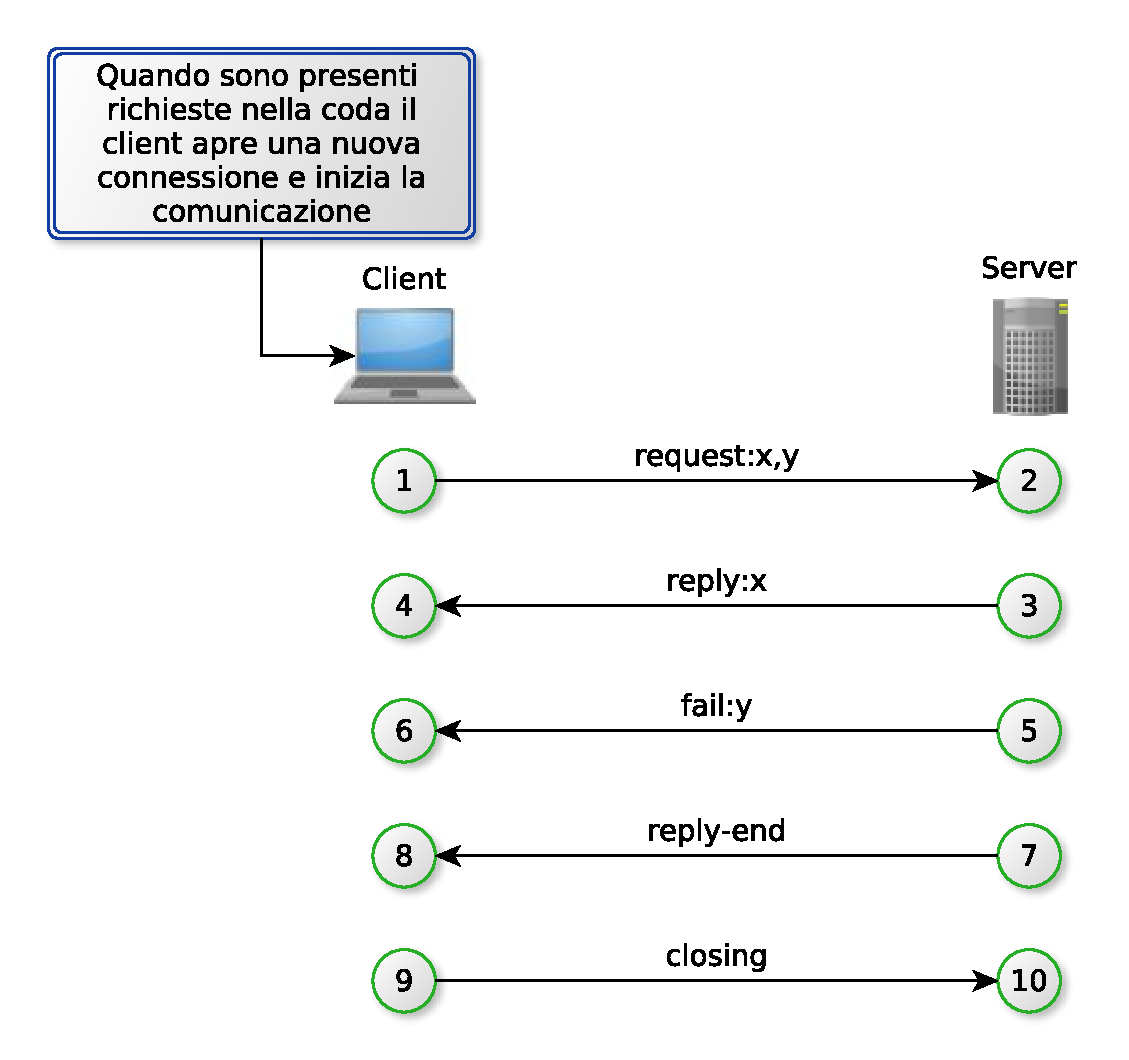
\includegraphics[width=10cm]{Immagini/InterazioniClientServer}
\caption{Esempio dello schema implementato per l'interazione tra client e server.\label{f:clientserverinteraction}} 
\end{center} 
\end{figure}

La gestione della comunicazione e dello schema di interazione viene effettuata tramite una macchina a stati specifica per client e server, le quali si occupano di leggere ed effettuare l'analisi logico-sintattica dei messaggi generando le eventuali risposte o semplicemente modificando lo stato interno della macchina stessa.

\begin{figure}
\begin{center}
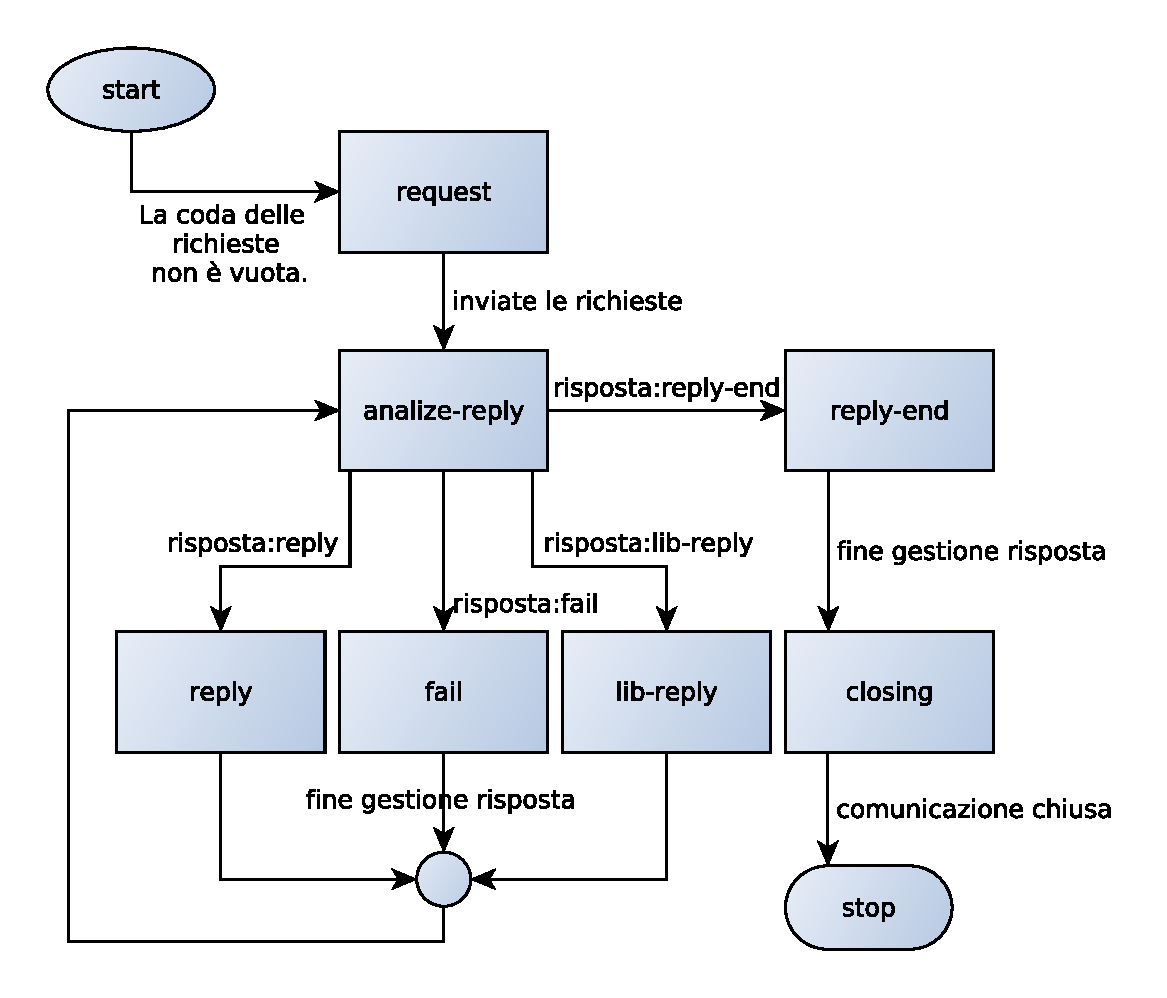
\includegraphics[width=11cm]{Immagini/StateMachineClient}
\caption{Diagramma a stati per la gestione della comunicazione delle richieste da parte del client.\label{f:stateclient}} 
\end{center} 
\end{figure}

Usare messaggi testuali per la comunicazione consente di semplificarne la gestione e rende possibile espandere il linguaggio semplicemente utilizzando nuove etichette, consentire tutto ci\`o ha per\`o reso necessario strutturare l'implementazione delle macchine a stati in modo che fossero altrettanto espandibili. Per far questo \`e stato preso come modello il pattern \textit{State}, descritto al paragrafo \ref{sub:state}, e la logica di ogni stato \`e stata incapsulata in un oggetto differente. Questo consente di espandere la macchina a stati semplicemente definendo nuovi oggetti i quali sono totalmente indipendenti dagli altri.

% TODO: rimandare alla classe protocol per la mappa del protocollo


I messaggi attualmente implementati sono:





\section{I Package java} 
\label{sec:sfrc_packages}
La classi che compongono il progetto sono suddivise in una serie di package. % TODO: decidere se la prossima frase va bene
Alcuni di questi sono pensati per rappresentare una possibile estensione a quelli forniti dal framework stesso e ne riproducono la struttura e le convenzioni sui nomi, gli altri sono librerie che affiancano il framework nella costruzione dell'applicazione.


%!TEX root = ../tesi.tex

\chapter{Test e Risultati}
\label{ch:testerisultati}

In questo capitolo vengono presentati e commentati i test effettuati sui moduli di libreria del progetto.

Nella sezione \ref{sec:strutturatest} viene presentata la struttura dell'impianto di test, sia da lato client che da lato server.
Successivamente, nella sezione \ref{sec:test}, vengono mostrati i risultati dell'esecuzione di alcuni test particolarmente significativi. 
Infine nella sezione \ref{sec:correlate} vi \`e la descrizione di alcune attivit\`a correlate emerse durante lo sviluppo.


\section{Struttura dei test}
\label{sec:strutturatest}
La fase di testing del progetto ha verificato che il funzionamento dei meccanismi implementati all'interno dei moduli esplicati nel capitolo precedente producesse un corretto output visivo.

Oltre a ci\`o questa fase ha avuto l'obbiettivo di riprodurre i test presenti all'interno del progetto \textbf{SF20LiteTestWorld}, che consiste in un modulo di estensione del framework volto a semplificare la gestione delle finestre grafiche nelle applicazioni. Questo modulo \`e in via di sviluppo e per questo non \`e ancora parte integrante delle funzionalit\`a di base offerte dallo \ac{SF}. Tuttavia il codice relativo ad esso \`e disponibile alla stessa fonte della versione del framework indicata al paragrafo \ref{sub:sfsource}.
I test presenti in \textbf{SF20LiteTestWorld} sono stati pensati non solo per verificare la correttezza delle funzionalit\`a, ma anche per mostrare alcune delle capacit\`a del framework stesso.

Per evitare un'eccessiva duplicazione del codice le classi di implementazione dei test, sia lato client che lato server, sfruttano l'ereditariet\`a da una classe genitore comune per condividere tutte le parti comuni.

In figura \ref{f:abstractclient} possiamo vedere la gerarchia delle classi dei client di test. Per implementare un qualsiasi test \`e sufficiente creare una sottoclasse di \texttt{AbstractClient} e implementare al suo interno i metodi astratti della classe genitore. 
\begin{figure}
\begin{center}
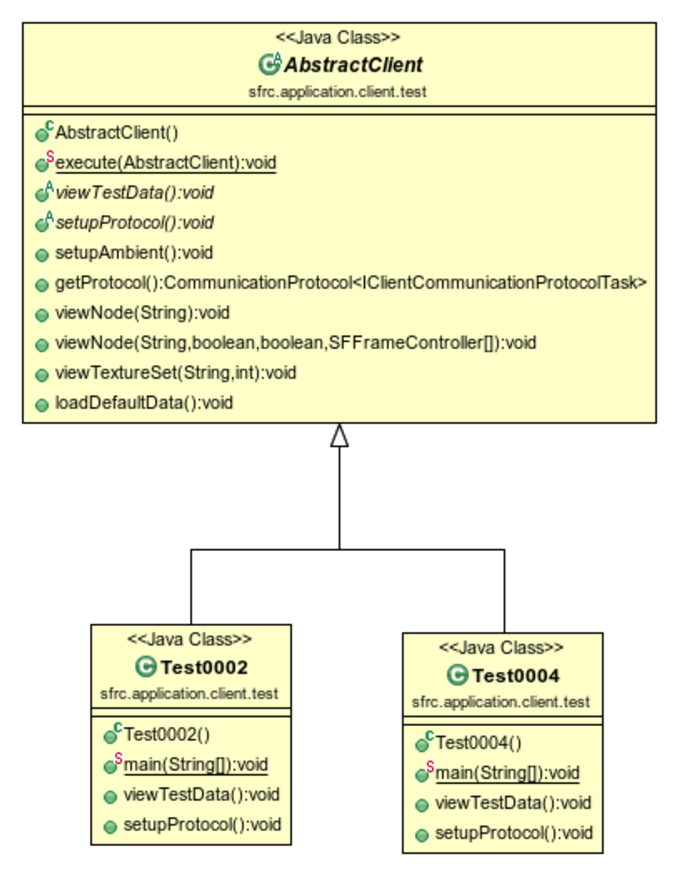
\includegraphics[scale=0.85]{Immagini/abstractclient}
\caption{Gerarchia delle classi di implementazione dei client.\label{f:abstractclient}} 
\end{center} 
\end{figure}
In maniera del tutto simile \`e possibile vedere in figura \ref{f:abstractserver} lo stesso principio applicato per l'implementazione di differenti server di test. Questi, opportunamente configurati, vengono usati per riprodurre le diverse condizioni a cui il client pu\`o essere sottoposto durante la comunicazione, ad esempio generando dei ritardi di risposta o l'assenza di alcuni dati.
\begin{figure}[t]
\begin{center}
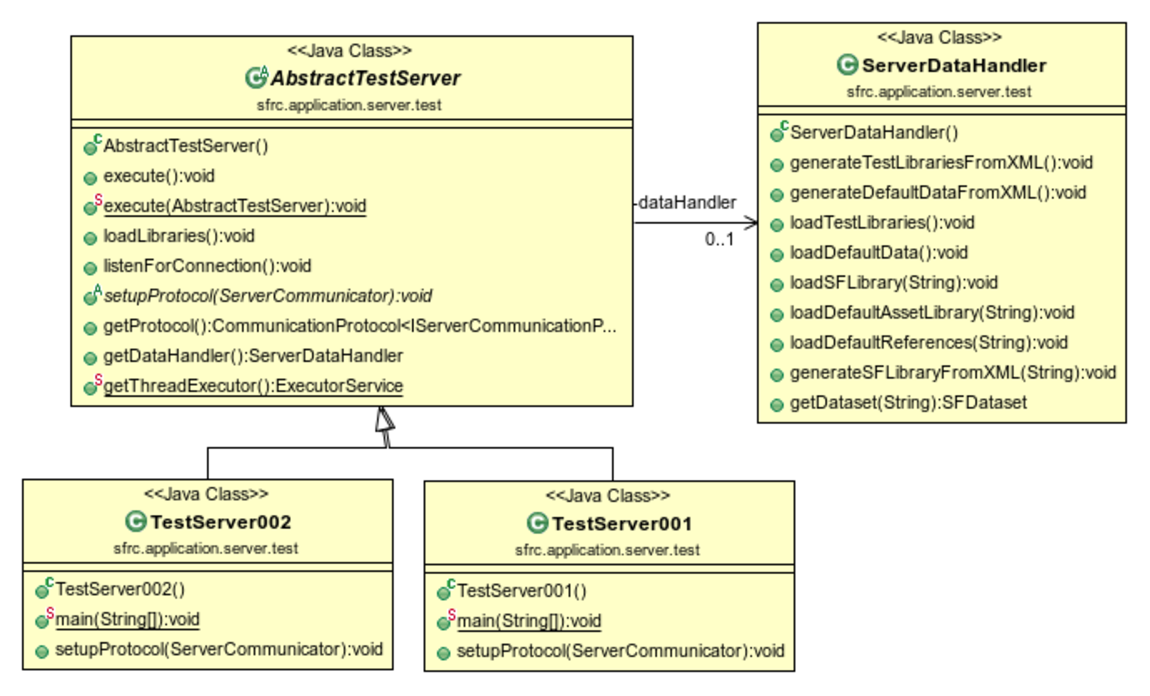
\includegraphics[scale=0.75]{Immagini/abstractserver}
\caption{Gerarchia delle classi di implementazione dei server.\label{f:abstractserver}} 
\end{center} 
\end{figure}
In quest'ultima figura \`e evidenziata la classe \texttt{ServerDataHandler}, la quale si occupa di effettuare la gestione dei dati sul server in esecuzione. Non essendoci la necessit\`a di renderizzare i dati tridimensionali, non \`e richiesta un'infrastruttura centralizzata complessa come quella del DataCenter del framework.

Le classi che implementano i test sono contenute nei package \\\texttt{sfrc.application.client.test} e \texttt{sfrc.application.server.test}.

\section{Test significativi}
\label{sec:test}
Il server di test utilizzato nelle prove descritte di seguito \`e il \textbf{TestServer002} ed \`e stato configurato per avere $3$ secondi di ritardo tra la risposta ad una richiesta ed un'altra. Questa configurazione permette di osservare nel dettaglio la reazione dei meccanismi implementati ad un arrivo progressivo dei dati.

\subsection{Test0006}
Questo test ha l'obbiettivo di visualizzare all'interno di una finestra, tre oggetti che condividono una geometria dalla forma di fungo e su cui sono applicate delle texture. Sia la geometria che le texture sono generate proceduralmente durante l'esecuzione usando la capacit\`a di calcolo della \ac{GPU}.
\begin{figure}%[t]
\begin{center}
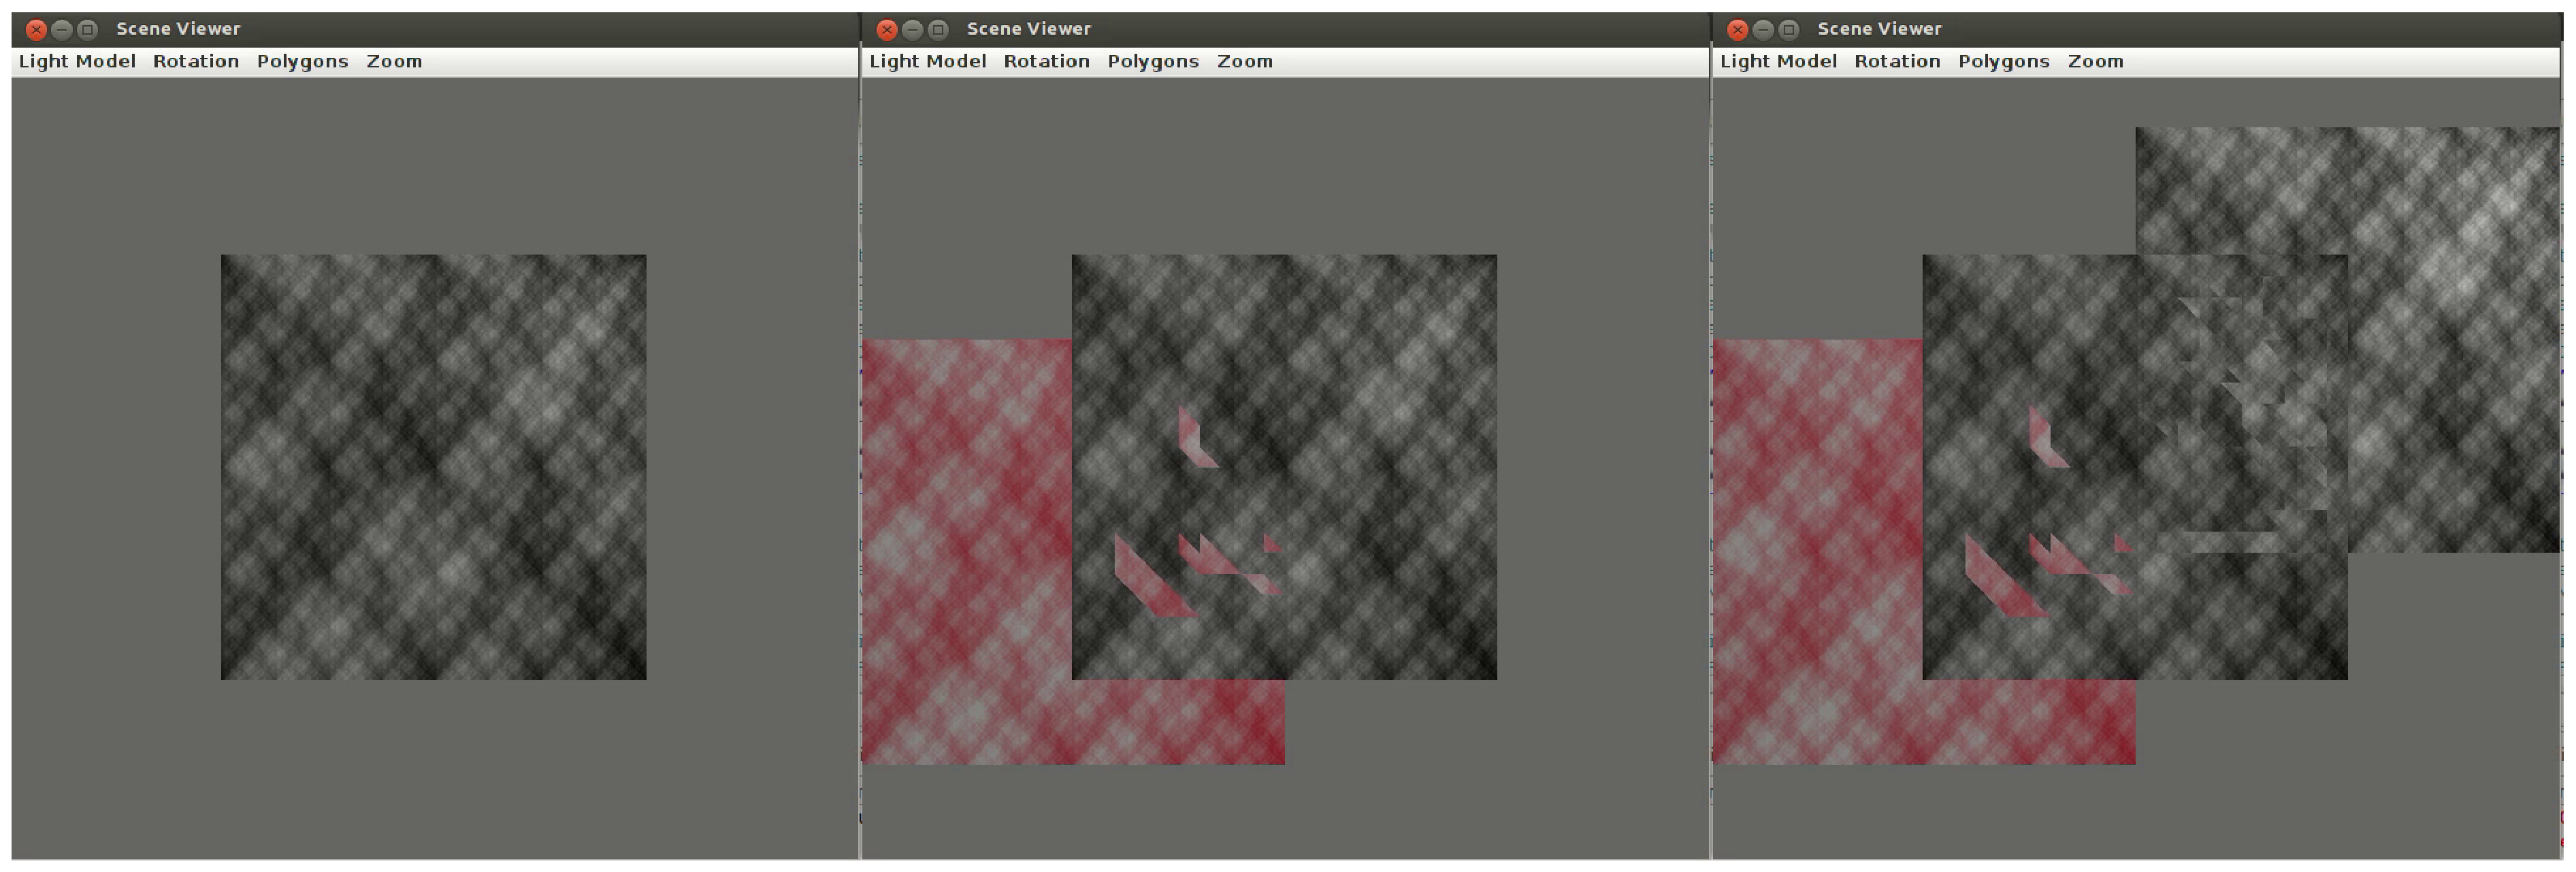
\includegraphics[width=\textwidth]{Immagini/test0006/test0006-wall1}
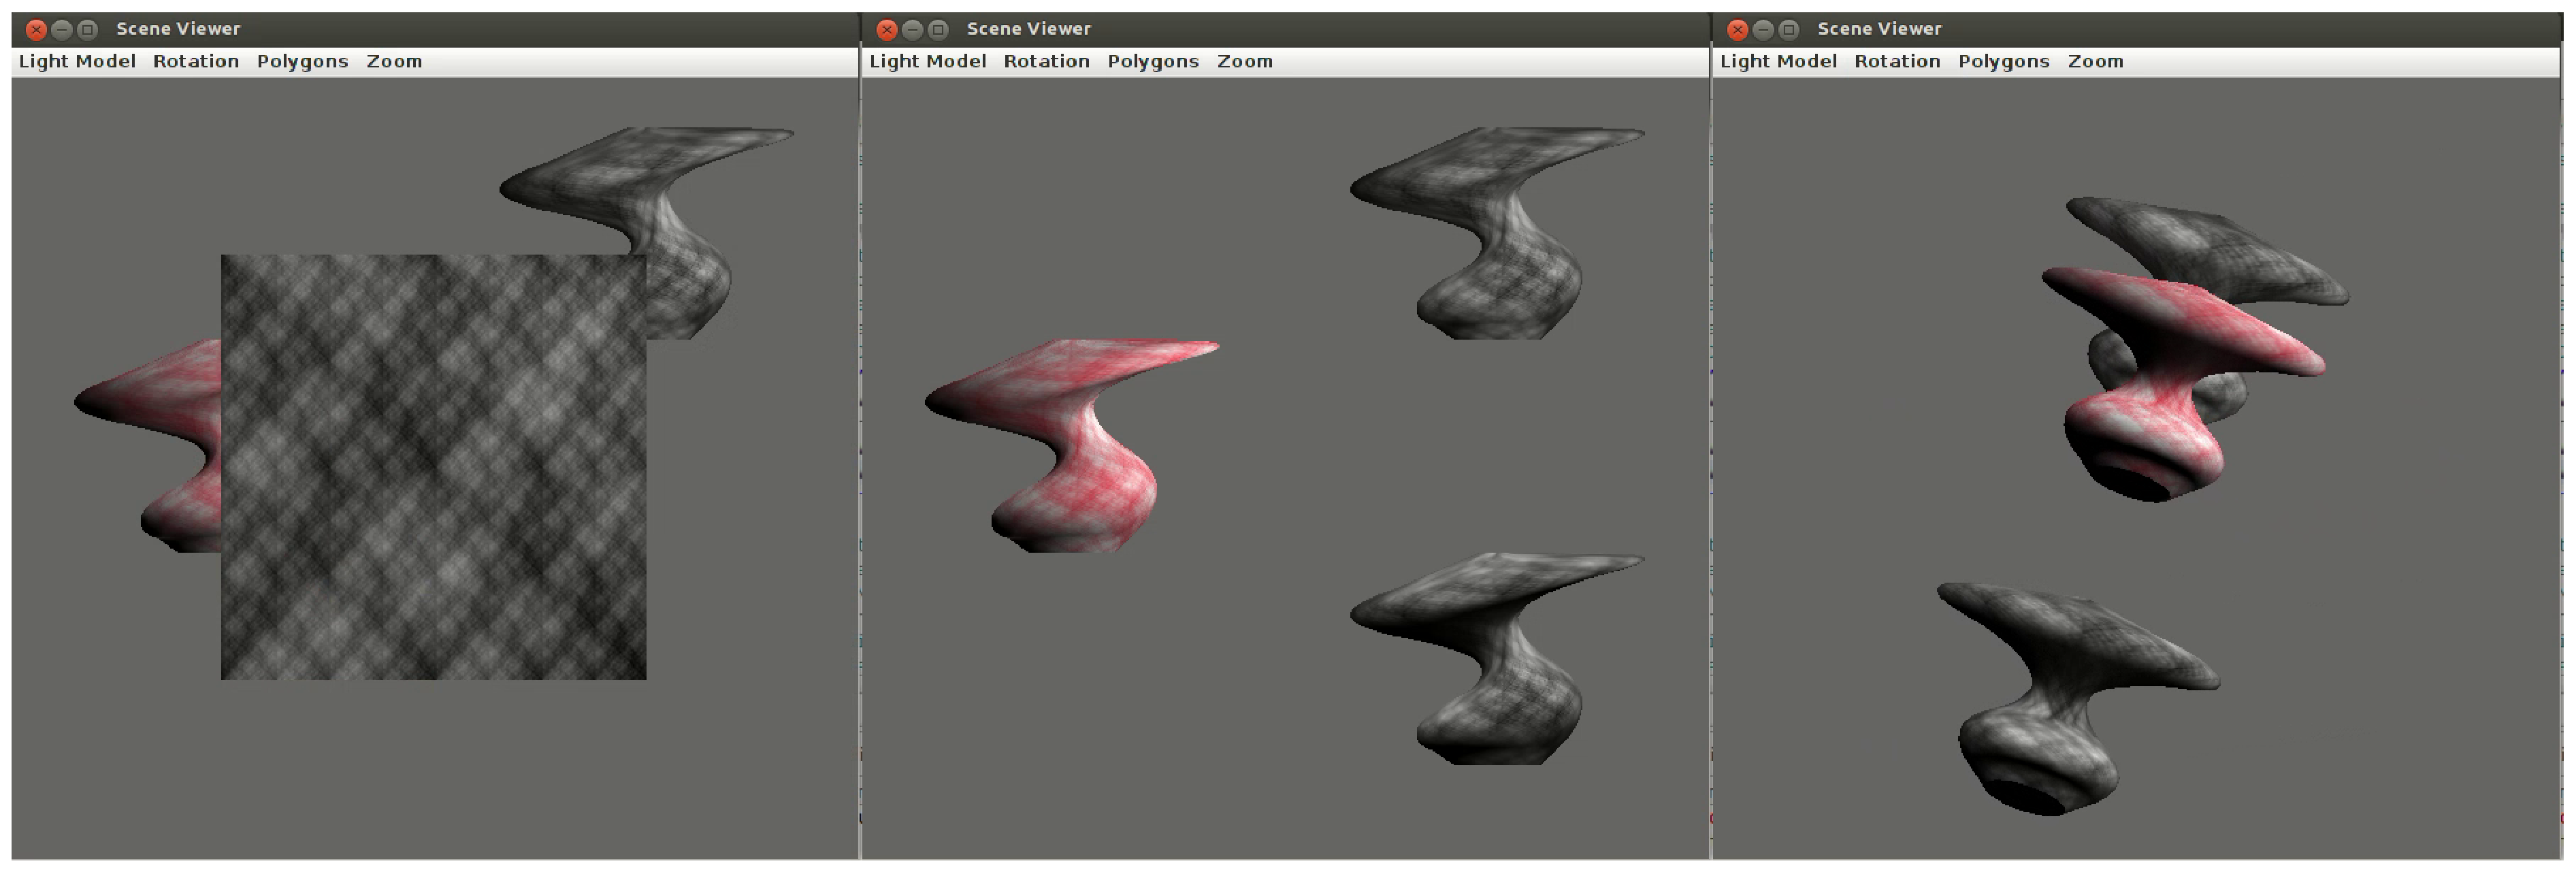
\includegraphics[width=\textwidth]{Immagini/test0006/test0006-wall2}
\caption{Fotogrammi estratti dall'esecuzione del test Test0006. \label{f:test0006-wall}} 
\end{center} 
\end{figure}
In figura \ref{f:test0006-wall} viene mostrata una sequenza di fotogrammi dell'esecuzione del test: al lancio dell'applicazione (fig.\ref{f:test0006-wall} in alto a sinistra) la scena richiesta viene temporaneamente sostituita con un'altra che contiene un semplice cubo texturizzato. 
Al loro arrivo, i dati della scena reale che contengono i riferimenti ai tre oggetti vengono analizzati generando la richiesta degli oggetti verso il server. Nel frattempo ognuno di essi viene sostituito con un cubo posto al centro della scena. La sostituzione non genera un cambiamento visibile in quanto i tre cubi sono sovrapposti e posizionati esattamente come quello contenuto nella scena sostitutiva.

Quando i dati del primo oggetto vengono ricevuti (fig.\ref{f:test0006-wall} in alto al centro) vengono immediatamente applicati alla scena: possiamo notare il cambiamento di colore e la traslazione di un cubo verso sinistra. 
L'oggetto non cambia forma perch\'e il pacchetto di informazioni contiene un riferimento alla geometria ``fungo'' generica ancora non presente e per cui viene generata una richiesta. 
Nel fotogramma successivo (fig.\ref{f:test0006-wall} in alto a destra) vediamo gli effetti dell'arrivo del pacchetto di informazioni relativo al secondo oggetto: un altro cubo viene traslato, stavolta verso destra. 
L'informazione sulla geometria ``fungo'' non \`e ancora arrivata, ma non viene generata una nuova richiesta dato che il sistema ha gi\`a una richiesta pendente, l'oggetto viene invece registrato per un update della geometria.
Nel quarto fotogramma (fig.\ref{f:test0006-wall} in basso a sinistra), viene ricevuta la geometria e tutti gli oggetti che si erano registrati per un update vengono aggiornati. Non avendo ancora ricevuto i dati relativi al terzo oggetto, esso rimane nella sua forma sostitutiva. Questo accade a causa del parallelismo dei processi che effettuano le richieste, il quale consente di non dover necessariamente ricevere i dati in un ordine specifico.
Nella penultima immagine (fig.\ref{f:test0006-wall} in basso al centro) si vede l'aggiornamento visivo all'arrivo delle informazioni sul terzo oggetto. Avendo gi\`a ricevuto i dati della geometria essa viene applicata immediatamente insieme alla traslazione. Nell'ultimo fotogramma vediamo la scena finale ruotata dai controlli della finestra client. Per effettuare la navigazione della scena non \`e pi\`u necessario richiedere altri dati al server e le connessioni vengono chiuse. In figura \ref{f:schemadati} sono rappresentate le relazioni tra i dati durante l'esecuzione del test.
\begin{figure}
\begin{center}
\includegraphics[width=\textwidth]{Immagini/schemadati}
\caption{Schema delle relazioni interne tra i dati del Test0006.\label{f:schemadati}} 
\end{center} 
\end{figure}

Per non appesantire la precedente descrizione si \`e omesso che durante l'esecuzione sono stati richiesti e trasferiti anche i dati relativi alle texture da applicare ai modelli. La transizione non \`e direttamente visibile dato che le texture sostitutive hanno la stessa trama e non sono visivamente distinguibili.

\subsection{Test0019}
Questo test prevede la visualizzazione di un oggetto avente geometria a fungo a cui viene applicata una texture e una \textit{bump map}\footnote{Una bump map \`e un particolare tipo di texture che viene utilizzata tramite la tecnica del \textit{Bump Mapping}. Questa tecnica si serve delle informazioni della bump map per descrivere la variazione da applicare al vettore normale di ogni punto di una superficie a cui \`e applicata. Ci\`o permette di ottenere l'effetto visivo di superfici irregolari senza spostare i vertici della superficie stessa}. Anche in questo caso sia la geometria che le texture sono ottenute proceduralmente attraverso il rendering della \ac{GPU}.
\begin{figure}%[t]
\begin{center}
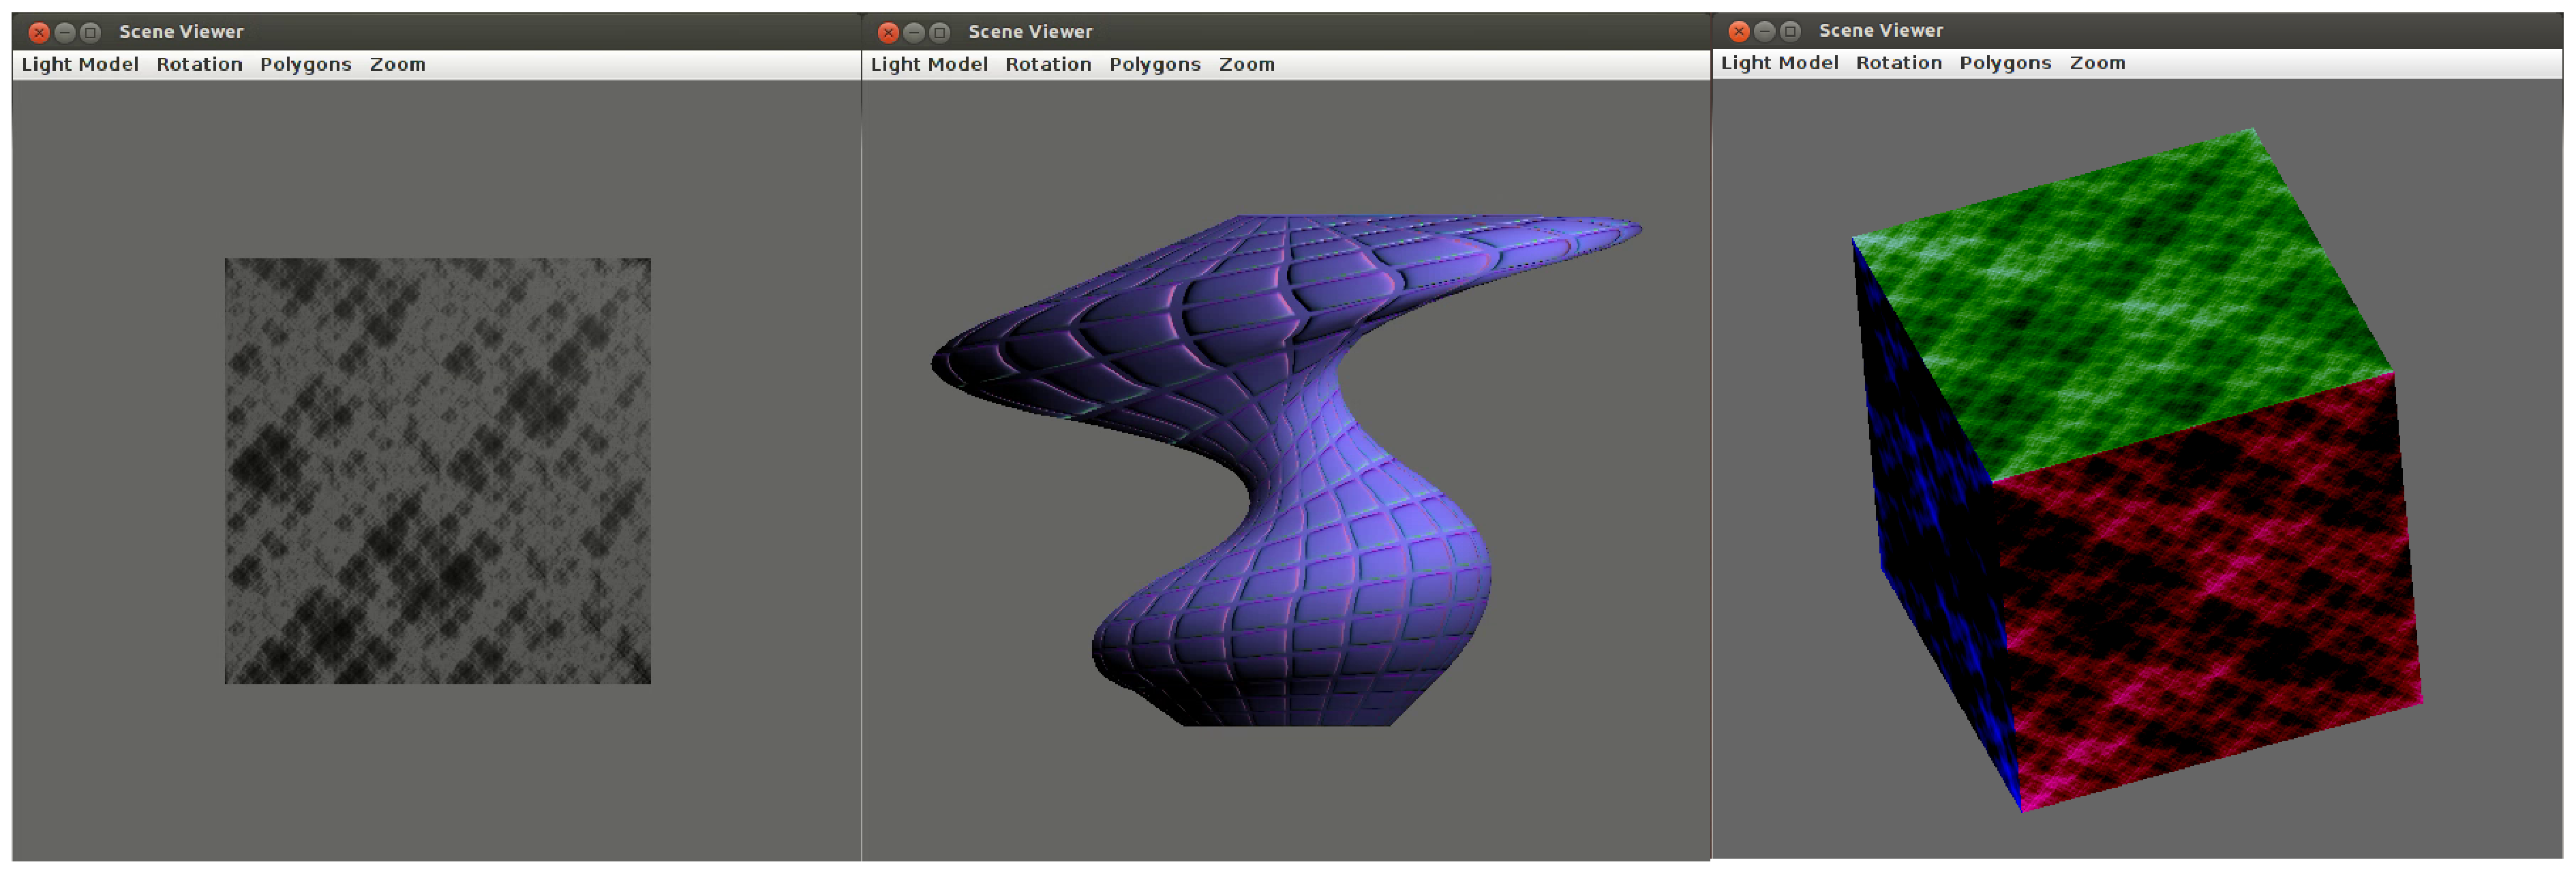
\includegraphics[width=\textwidth]{Immagini/test0019/test0019-wall1}
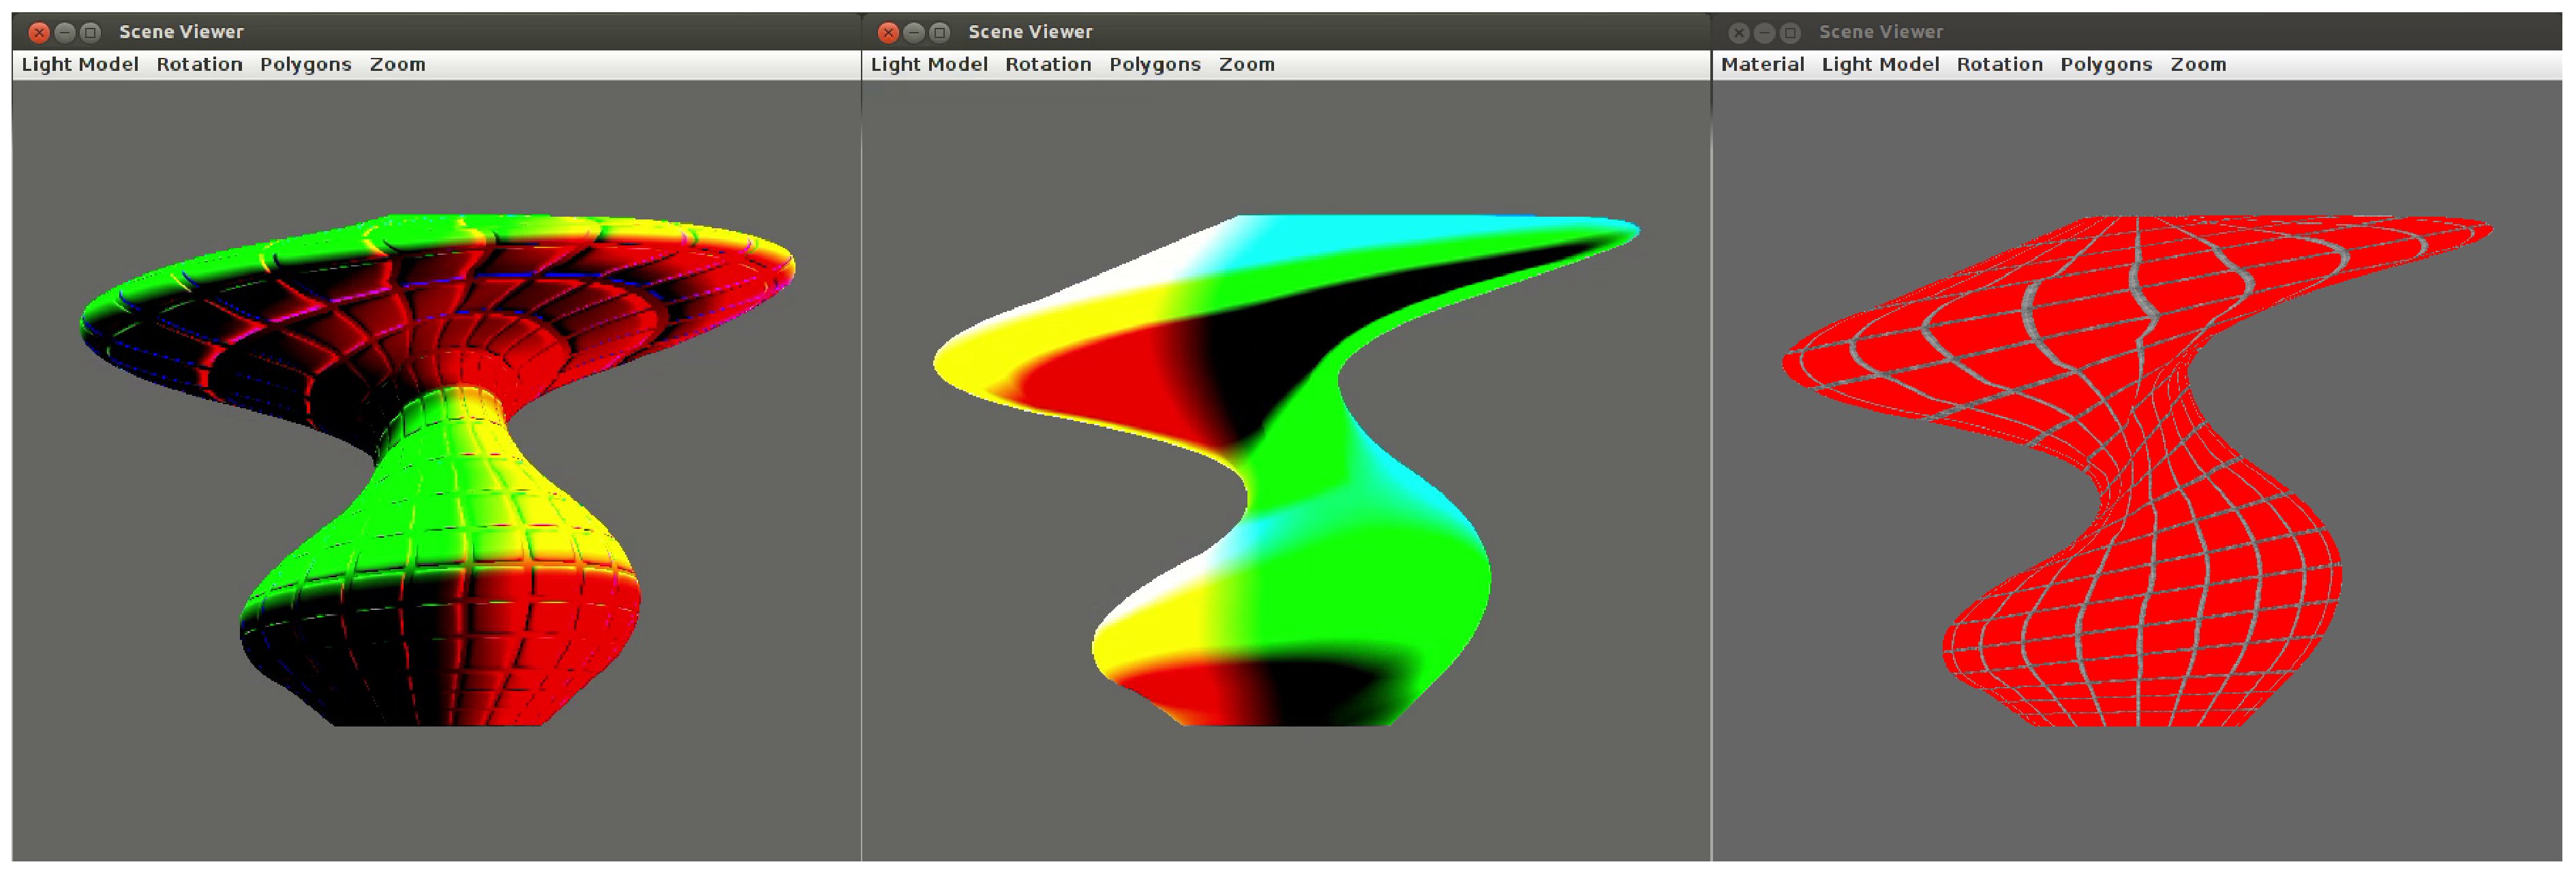
\includegraphics[width=\textwidth]{Immagini/test0019/test0019-wall2}
\caption{Fotogrammi estratti dall'esecuzione del test Test0019. \label{f:test0019-wall}} 
\end{center} 
\end{figure}
Nei primi due fotogrammi in alto a sinistra della figura \ref{f:test0019-wall} vediamo le immagini della geometria sostitutiva (il cubo) e dell'oggetto reale della scena richiesta, anche in questo caso un fungo. L'obbiettivo del test \`e verificare che l'effetto di Bump Mapping venga applicato correttamente alla geometria del fungo una volta che essa viene ottenuta tramite la connessione.
Nella seconda immagine si pu\`o infatti notare l'effetto ``piastrellato'' sulla superficie dell'oggetto. Sebbene dalla prima immagine non sia ben distinguibile, anche il cubo sostitutivo fa uso di questa tecnica: nel terzo fotogramma (fig.\ref{f:test0019-wall} in alto a destra) esso viene disegnato in modo che ogni punto della sua superficie sia di un colore diverso in base alla direzione del vettore normale al punto stesso. Le facce, pur essendo piatte, non hanno un colore uniforme mostrando la corretta applicazione della tecnica. Il quarto fotogramma (fig.\ref{f:test0019-wall} in basso a sinistra) illustra lo stesso effetto applicato al fungo: a un colore diverso sulla superficie corrisponde una normale puntata in una diversa direzione. Gli ultimi due fotogrammi mostrano rispettivamente la geometria finale, colorata in base alla direzione della luce senza tener conto delle normali, e la geometria colorata applicando la texture in modo piatto senza illuminazione.

\begin{figure}
\begin{center}
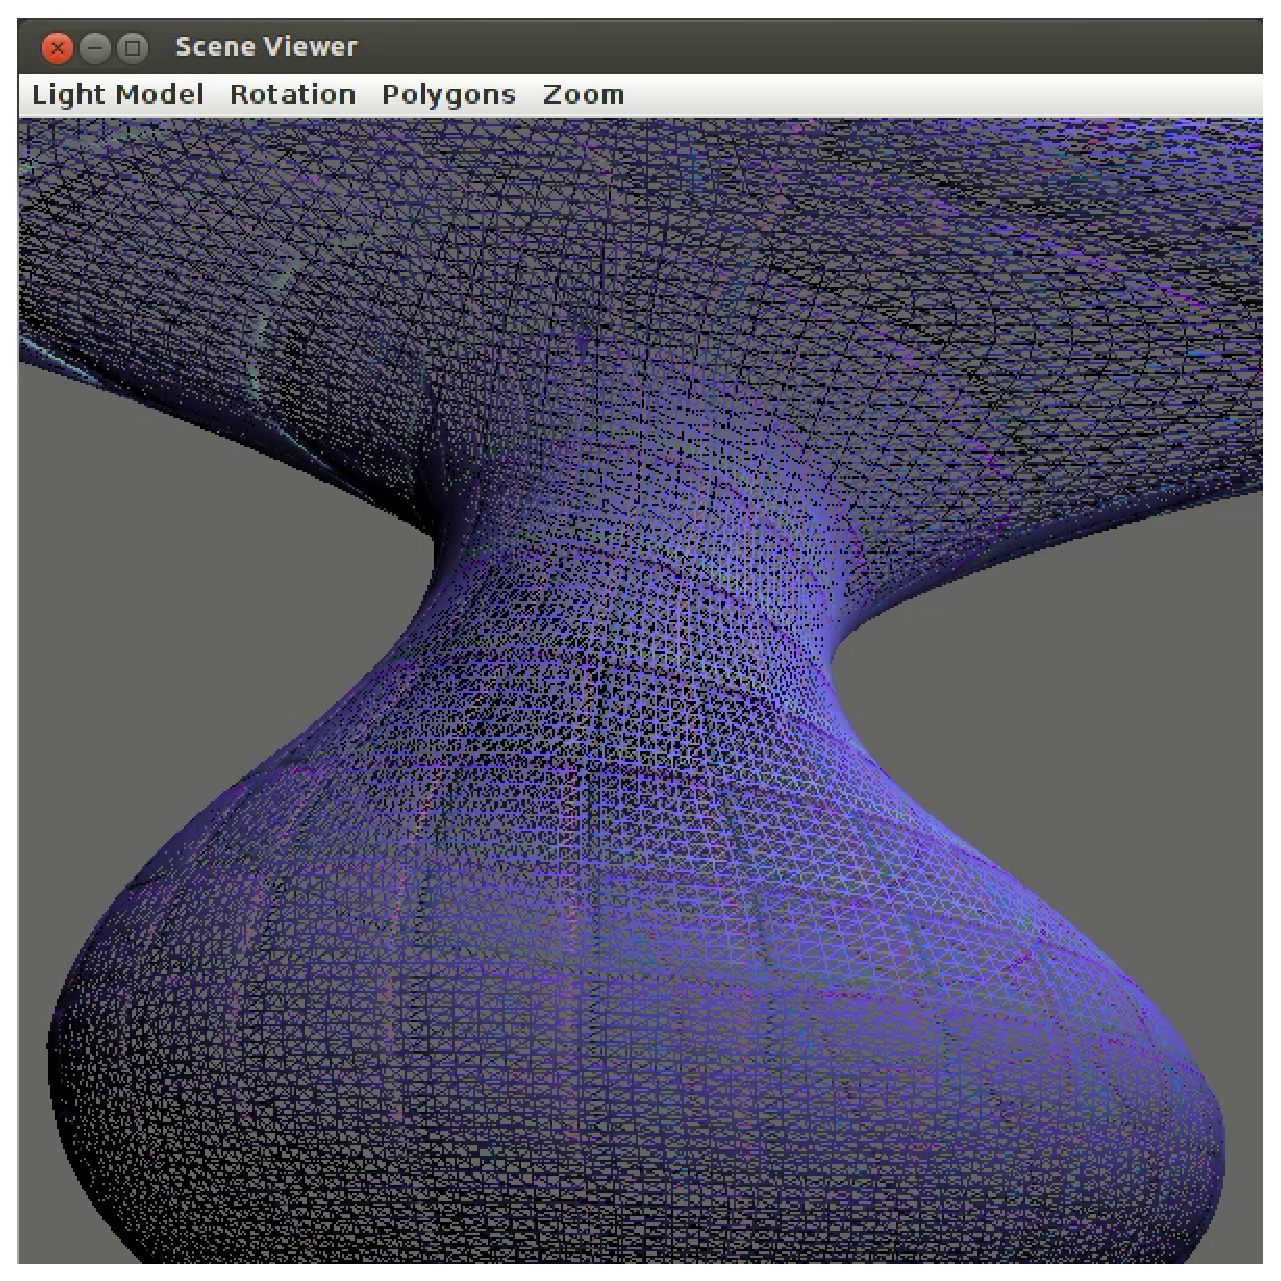
\includegraphics[width=10cm]{Immagini/test0019/test0019-tessel}
\caption[Tassellazione della geometria usata nel Test0019.]{Particolare di un fotogramma estratto dall'esecuzione del test Test0019, \`e posta in evidenza la tassellazione in triangoli operata sul modello del fungo. \label{f:test0019-tessel}} 
\end{center} 
\end{figure}
Come esplicato la tecnica applicata non effettua una reale traslazione dei vertici della geometria, in figura \ref{f:test0019-tessel} vediamo messo in risalto questo particolare grazie ad uno zoom ravvicinato. Con questa immagine possiamo vedere anche il livello di tassellazione della geometria generata dalla pipeline programmabile.

\section{Attivit\`a correlate}
\label{sec:correlate}
La variet\`a dei contenuti dei test di riferimento ha reso necessario un lavoro aggiuntivo dedicato alla creazione di un insieme di Dataset sostitutivi da inserire nella libreria di oggetti di default, usati come rimpiazzo temporaneo.
Questa libreria \`e stata realizzata progressivamente durante l'implementazione dei test, quando si rendeva necessaria la costruzione di un Dataset specifico e quelli gi\`a realizzati erano di tipo incompatibile.
Queste incompatibilit\`a dipendono da ci\`o che i Dataset rappresentano: geometrie, texture, etc. 

Oltre a ci\`o \`e stato necessario implementare un metodo pratico per definire la lista di Dataset sostitutivi con cui effettuare gli scambi. La sola creazione della classe \texttt{SFDatasetReplacement} rendeva necessario definire a runtime la lista, che poteva essere memorizzata solamente in un file binario non leggibile ne modificabile senza un apposito tool. Per risolvere il problema \`e stato modificato il modulo di lettura/scrittura dei file xml preesistente nel framework, aggiungendo la capacit\`a di codificare e decodificare i dati contenuti in un \texttt{SFDatasetReplacement}. 
La lista dei sostituti \`e cos{\`\i} editabile a mano modificando un file testuale xml chiaramente leggibile (figura \ref{f:listaxml}).

\begin{figure}
\begin{center}
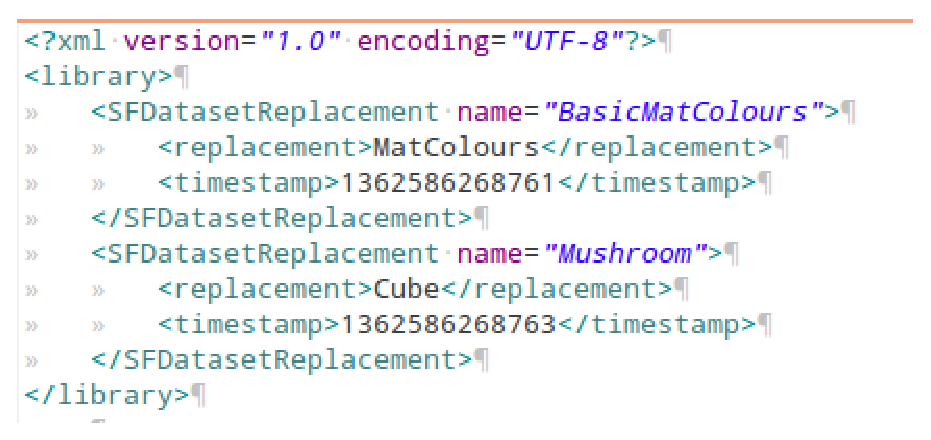
\includegraphics[width=10cm]{Immagini/listaxml}
\caption{File xml della lista di sostituzione.\label{f:listaxml}} 
\end{center} 
\end{figure}
%!TEX root = ../tesi.tex

\chapter{Conclusioni}
\label{ch:conclusioni}
L'obbiettivo del progetto di tesi \`e stato quello di progettare e produrre una serie di moduli software di supporto per lo sviluppo di applicazioni di grafica tridimensionale orientate al Web, che fanno uso dello Shadow Framework. I moduli prodotti si sono dimostrati efficaci allo scopo, consentendo di riprodurre i test effettuati con dati grafici in locale anche nella condizione in cui i dati sono memorizzati su di un server remoto. 
Per consentire la parallelizzazione delle richieste sono stati affrontati numerosi problemi di sincronizzazione per cui \`e stato di fondamentale importanza acquisire familiarit\`a la programmazione multi-thread in Java.


Il lavoro di progettazione e sviluppo del codice \`e stato guidato dai principi di riutilizzo e modularit\`a, sfruttando pratiche quali i \textit{Design Pattern} e le metodologie di sviluppo agile.



\section{Sviluppi futuri}
I possibili sviluppi futuri del lavoro compiuto durante questa tesi sono molteplici e orientati in diverse direzioni. Innanzitutto vi \`e la possibilit\`a di espandere i moduli \textbf{Client} e \textbf{Server} in modo che al loro interno vi siano degli strumenti per gestire in modo pi\`u completo le sessioni di comunicazione. Con questo si intende la possibilit\`a di instaurare una comunicazione non legata strettamente alle richieste di dati, ma orientata allo scambio di messaggi di controllo, in modo di consentire l'interazione di utenti differenti che condividono la stessa simulazione.

Un'altra possibilit\`a di sviluppo consiste nell'integrare nel modulo \textbf{Base Communication} lo sfruttamento di protocolli di comunicazione pi\`u complessi e potenti, come ad esempio il protocollo peer-to-peer sfruttato nella tesi \cite{tesi:truzzi}.

La possibilit\`a di editare via xml le liste di sostituzione dei dataset non eliminano il problema che la loro produzione sia lunga e laboriosa, soprattutto quando gli scenari diventano ricchi di modelli tridimensionali. Per questo motivo sarebbe necessario un tool in grado di esaminare i file che descrivono gli scenari e generare in automatico la lista.

\`E in fase di realizzazione un'estensione del protocollo di comunicazione che consenta al server di rispondere alle richieste con una libreria contenente un insieme di Dataset.

Oltre agli sviluppi direttamente collegati al progetto di tesi, i test effettuati hanno evidenziato una serie di elementi del framework che potrebbero avere la necessit\`a di correzioni.

% TODO: eliminare i dettagli ed espandere il generico.

%%!TEX root = ../tesi.tex

% NOME PROVVISORIO
Appunti sparsi sul progetto

% cambiare titolo
\section{Infrastruttura di rete} 
\label{sub:rete}
Date le specifiche iniziali esposte nel capitolo \ref{ch:introduzione}, una parte fondamentale del progetto è stata decidere quale infrastruttura per la comunicazione di rete sfruttare per poter utilizzare e testare il modulo \textbf{RemoteDataCenter Tool}, che si occupa della gestione delle richieste di Dataset.

Se da lato client è ovvia la necessità di sviluppare uno strato dell'applicazione che si occupa della comunicazione di rete, da lato server si sono presentate diverse possibilità: 
\begin{enumerate}
	\item  utilizzare un file server che permettesse semplicemente di accedere ai file contenti i dati tramite la rete;
	\item  utilizzare un application server java, come Tomcat o Glassfish, a cui un'applicazione client potesse connettersi e che attraverso l'esecuzione di servlet realizzasse il trasferimento dei dati da server a client;
	\item  utilizzare un'applicazione server ad hoc appositamente sviluppata;
\end{enumerate}

La prima soluzione è probabilmente la più semplice, ma la meno flessibile dato che consente solo di un accesso diretto ai file di descrizione dei dati senza alcuna possibilità di un'elaborazione lato server e spostando tutto il peso di un'eventuale interazione tra client direttamente su quest'ultimi.

La seconda soluzione offre più possibilità e flessibilità rispetto alla prima: l'utilizzo di un application server java mette a disposizione una piattaforma che consente una pre-elaborazione dei dati lato server e che possiede direttamente una serie di componenti per la gestione di compiti complessi legati alle sessioni degli utenti, come ad esempio l'autenticazione e la sicurezza. Nonostante i pregi, questo tipo di soluzione possiede anche lati negativi: gli application server generici non sono sviluppati per questo tipo di applicazioni e non era garantita una flessibilità sufficiente per cui all'aumentare della complessità del progetto e delle sue esigenze non fosse necessario abbandonare l'architettura. 

La terza soluzione è sicuramente la più flessibile ed estendibile dato che, se necessario, consente di modificare direttamente il server per adattarsi alle esigenze dell'applicazione. Lo svantaggio è la necessità di dover implementare da zero tutte quelle funzionalità non solo di comunicazione, ma anche di autenticazione o di sicurezza che una soluzione già pronta potrebbe possedere nativamente.

Nella scelta tra le tre soluzioni hanno pesato prevalentemente la volontà di realizzare un'architettura funzionante con la scrittura di meno codice possibile e quella di mantenere una bassa complessità iniziale che non penalizzasse però un'estensione futura delle funzionalità. In quest'ottica la prima soluzione è stata anche la prima ad essere scartata, perché sebbene garantisse un tempo di messa in opera molto basso non consente un'estensione di funzionalità. 
La scelta finale è ricaduta sulla terza soluzione che pur costringendo a rinunciare alle funzionalità avanzate della seconda, elimina difficoltà e tempistiche di una installazione e configurazione dell'application server. Inoltre, limitando inizialmente lo sviluppo a funzionalità di base, è possibile limitare la complessità del codice ad un livello non molto più elevato rispetto alla seconda soluzione.

%\chapter*{TMP}
\label{tmp}
Pluto
\section{tmp1}
Topolino
\subsection{tmp2}
Paperino
\subsubsection{tmp3}
Qui
\paragraph{tmp4}
Quo
\subparagraph{tmp5}
Qua

%----------------------------------------------------------
%	
%----------------------------------------------------------
\chapter{Gestione dei dati}
\label{ch:gestdati}
%----------------------------------------------------------
%	roba da cambiare
Data management is an important task in the Framework. Through an abstract data layer, any module of the framework can be stored in datafile or transfered to datastream and loaded at any time. 
%----------------------------------------------------------

\section{Il package shadow.system.data}
Questo package contiene una serie di classi ed interfacce base su cui si basa l'astrazione dei dati del framework.

\subsection{SFDataCenter}
Il \textbf{DataCenter} \'e il nodo fondamentale della gestione dei dati all'interno del framework. \'E un \textit{singleton}

\subsubsection{tmp3}
Qui
\paragraph{tmp4}
Quo
\subparagraph{tmp5}
Qua





%----------------------------------------------------------
%	Appendici
%----------------------------------------------------------
\appendix
%!TEX root = ../tesi.tex

% TODO: inserire le versioni dei software
\chapter{Note sul Software}
\label{a:notesoftware}

\section{Codice sorgente del progetto SF-Remote-Connection}
\label{sec:sfrcsource}
Il progetto SF-Remote-Connection \`e una libreria di classi java ospitate, al momento della scrittura di questo documento, sul portale Google Code per la condivisione di codice open source all'indirizzo \url{http://code.google.com/p/sf-remote-connection/}.
Il codice \`e attualmente rilasciato sotto licenza GNU GPL v3.

\section{Versioni dei software utilizzati}
\label{sec:versionisw}

\subsection{Shadow Framework 2.0}
\label{sub:sfsource}
La versione di riferimento del framework \`e disponibile all'indirizzo \url{http://code.google.com/p/shadowframework20lite/}. Il codice \`e attualmente rilasciato sotto licenza GNU GPL v3.

La revisione utilizzata \`e la: r201.

\subsection{JOGL}
\label{sub:jogl}
JOGL \`e un binding Java open source e multipiattaforma per l'\ac{API} grafica OpenGL.
I suoi sorgenti e i binari sono disponibili sul sito \url{http://jogamp.org/jogl/www/}.

La versione utilizzata \`e la build: 2.0-b66-20121101.

\subsection{Sviluppo del progetto}
\label{sub:sviluppo}
Nel corso del progetto sono stati usati questi strumenti software e linguaggi:
\begin{itemize}
	\item \textbf{Eclipse}, IDE versione Indigo Service Release 2 \cite{book:eclipse};
	\item \textbf{SVN}, tool di versioning \cite{book:svn};
	\item \textbf{Git}, tool di versioning \cite{site:git};
	\item \textbf{Java}, linguaggio di programmazione ad oggetti \cite{book:java};
\end{itemize}
Utili alla comprensione degli argomenti trattati sono stati i seguenti testi tecnici \cite{book:openglbible, book:librografica}

%!TEX root = ../tesi.tex

\chapter{Design Pattern}
\label{a:designpatterns}
Nel campo dell'Ingegneria del Software con Design Pattern si intende uno schema di progettazione del software utilizzato per risolvere un problema ricorrente.
Molti di questi schemi sono stai pensati per il paradigma di programmazione ad oggetti e descrivono, utilizzando ereditariet\`a e interfacce, le interazioni e relazioni tra oggetti e classi.

In questa appendice vengono esposte alcune note generali sui design pattern citati nel testo, sia che siano stati implementati direttamente o semplicemente coinvolti nello sviluppo del progetto di tesi perch\'e sfruttati dalle parti interessate del framework.
Nella trattazione viene descritto l'obbiettivo di ogni schema, l'utilit\`a, note implementative con schema \ac{UML} annesso e alcuni benefici della sua applicazione, vengono inoltre raggruppati per categoria cos{\`\i} come vengono presentati in \cite{book:designpattern}.

\section{Pattern Creazionali}
I pattern creazionali sono usati per creare un'astrazione sul processo di instanziazione degli oggetti, in modo da rendere il sistema indipendente da come gli oggetti vengono effettivamente creati. Questo tipo di pattern diviene importante quando un sistema dipende principalmente da oggetti composti da aggregati di componenti pi\`u piccole, rispetto ad oggetti gerarchici organizzati in base all'ereditariet\`a.

\subsection{Abstract Factory}
\label{sub:abstractfactory}
L'obbiettivo di questo pattern \`e fornire un'interfaccia per la creazione di famiglie di oggetti imparentati o dipendenti tra loro, eliminado la necessit\`a di specificare i nomi delle classi concrete all'interno del codice.

In questo modo un sistema pu\`o essere indipendente da come vengono creati gli oggetti concreti e pu\`o essere configurato per utilizzare diverse famiglie di oggetti a seconda delle necessit\`a. Un caso esemplificativo \`e quello di un tool per l'implementazione di interfacce grafiche che supporta diversi look-and-feel. L'utilizzo di un diverso look-and-feel comporta la definizione di una nuova famiglia di componenti grafiche le cui caratteristiche base sono per\`o fondamentalmente identiche: un pulsante pu\`o essere premuto e disegnato a schermo. L'applicazione dovrebbe essere appunto indipendente da come il pulsante viene istanziato, ma essere in grado di riconoscerlo per le sue funzionalit\`a.

\begin{figure}
\begin{center}
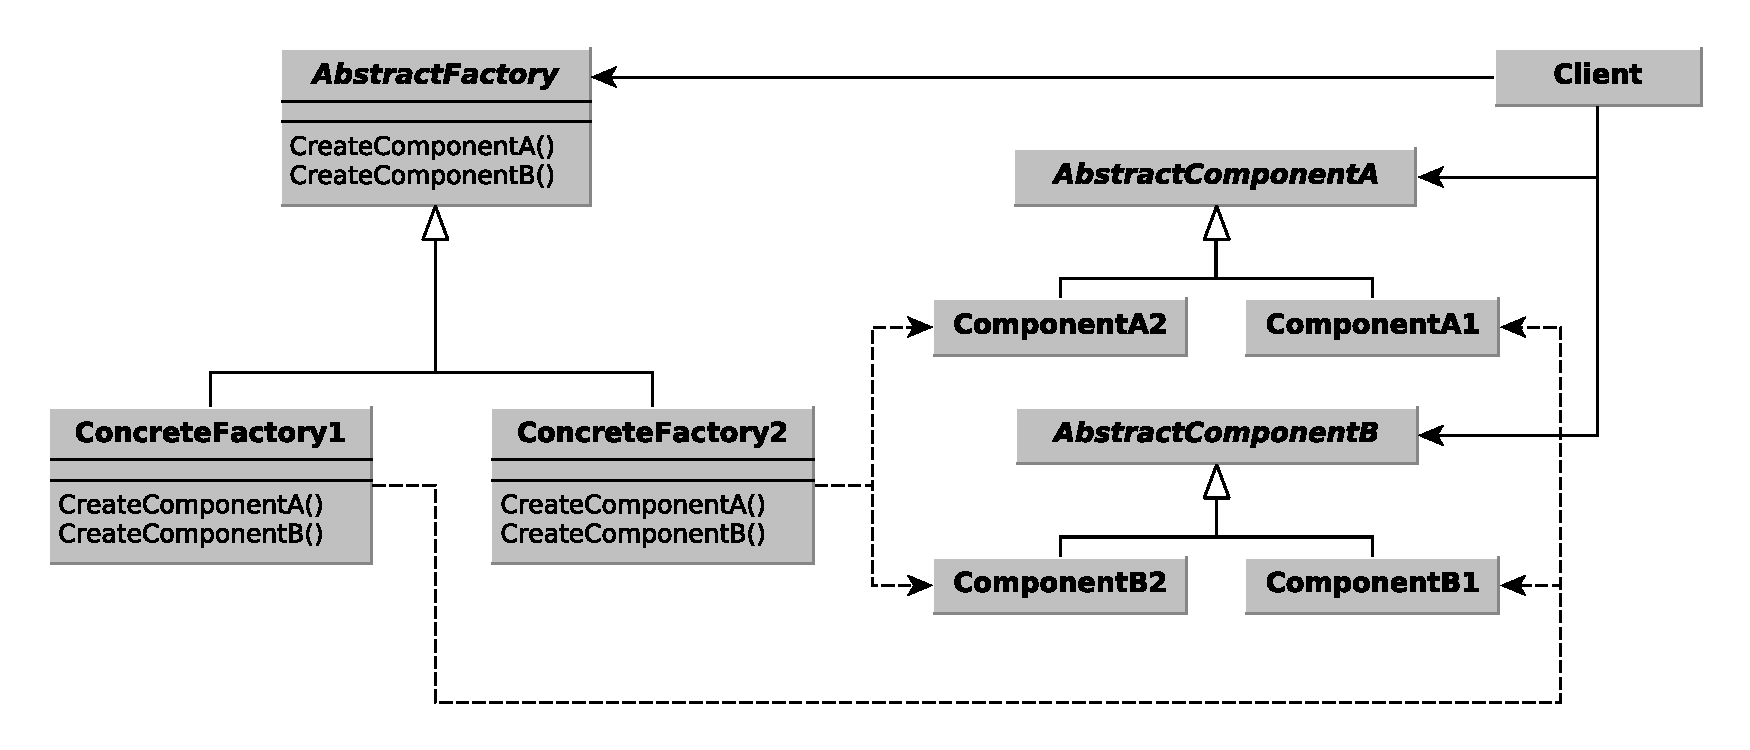
\includegraphics[width=13cm]{Immagini/AbstractFactoryPattern}
\caption{Struttura UML del pattern Abstract Factory.\label{f:abstractfactorypattern}} 
\end{center} 
\end{figure}

Per ottenere ci\`o \`e possibile definire una classe astratta o un'interfaccia differente per ogni componente generico desiderato, come \texttt{AbstractComponentA} e \texttt{AbstractComponentB} nella figura \ref{f:abstractfactorypattern}.
Si definisce poi una classe \texttt{AbstractFactory} astratta la cui funzione sia quella di creare istanze delle componenti astratte generiche. Se per ogni famiglia che si desidera implementare si generano sottoclassi concrete per ogni componente astratta e si definisce una Factory concreta in grado di istanziarle, come \texttt{ComponentA1} e \texttt{ConcreteFactory1} nell'esempio raffigurato, l'applicazione potr\`a utilizzare la Factory concreta che preferisce in modo del tutto indipendente da quale famiglia essa gestisce.

Questo schema permette di cambiare le famiglie di componenti in modo semplice e consente di isolare le classi concrete, dato che le componenti vengono utilizzate attraverso la loro interfaccia.

\subsection{Singleton}
\label{sub:singleton}
Lo scopo di questo pattern \`e garantire che di una determinata classe possa essere creata una unica istanza, fornendone un singolo punto di accesso globale.

L'utilit\`a di questo pattern \`e dovuta al fatto che spesso, all'interno di un'applicazione, ci sono servizi e funzionalit\`a condivise a cui deve essere associata una istanza univoca. Esempi classici in proposito sono il gestore del File System o il gestore dei servizi di stampa.

\begin{figure}
\begin{center}
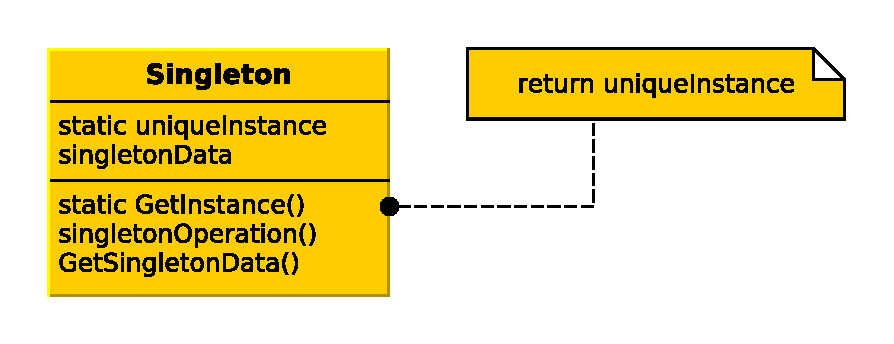
\includegraphics[width=12cm]{Immagini/SingletonPattern}
\caption{Struttura UML del pattern Singleton.\label{f:singletonpattern}}
\end{center} 
\end{figure}

Per ottenere questa propriet\`a spesso si delega alla classe stessa la responsabilit\`a di controllare la creazione delle propria istanza rendendo privato il suo costruttore, impedendo di fatto l'istanziazione dall'esterno. In figura \ref{f:singletonpattern} possiamo vedere lo schema \ac{UML} di una classe che utilizza il pattern in cui la classe possiede una unica istanza statica \texttt{uniqueIstance} accessibile solamente attraverso il metodo statico \texttt{GetInstance()}. 

Utilizzare questo schema consente di avere un pi\`u stretto controllo degli accessi alla risorsa, inoltre estendendo la classe \`e possibile raffinare le funzionalit\`a della risorsa e configurare l'applicazione a runtime per utilizzare l'istanza che serve per un caso specifico.

\section{Pattern Strutturali}
Questo tipo di pattern si occupa di come classi e oggetti vengono composte e interagiscono nella formazione di strutture pi\`u complesse. 
Un obbiettivo di questi pattern \`e permettere la composizione di oggetti complessi che uniscano le funzionalit\`a di moduli pi\`u piccoli rendendo quest'ultimi il pi\`u possibile riutilizzabili.

\subsection{Bridge}
\label{sub:bridge}
Questo pattern ha l'intento di disaccoppiare un'astrazione dalla sua implementazione in modo che entrambe possano evolversi in maniera indipendente.

Ci\`o \`e particolarmente utile quando si desidera evitare un legame permanente tra astrazione e implementazione, e si vuole permettere di scegliere o cambiare quest'ultima durante l'esecuzione. \'E utile inoltre quando sia astrazione che implementazione hanno la necessit\`a di essere estendibili attraverso sottoclassi. 

Un utile esempio per illustrare questo pattern \`e prendere in esame un ipotetico toolkit per interfacce grafiche, per renderlo il pi\`u possibile portabile su piattaforme diverse esso deve utilizzare un'astrazione che descriva le finestre in modo pi\`u generico possibile. Se per ottenere queste propriet\`a usassimo semplicemente una classe astratta \texttt{Window} da cui, usando l'ereditariet\`a, costruire sottoclassi specifiche per ogni sistema da supportare, otterremmo due svantaggi:
\begin{enumerate}
	\item Nell'evenienza di voler estendere la classe \texttt{Window} per coprire l'astrazione di altri tipi di finestra grafica esistente, per poter supportare tutte le piattaforme per cui esisteva una implementazione di \texttt{Window} dovremmo creare una sottoclasse specifica per ognuna di esse.
	\item Il codice del client diventa dipendente dalla piattaforma. Quando vi \`e la necessit\`a di creare una finestra, deve essere istanziata una classe concreta specifica e questo lega fortemente l'astrazione con l'implementazione utilizzata rendendo pi\`u complesso portare il codice del client su altre piattaforme.
\end{enumerate}
Per eludere questi problemi il pattern Bridge separa la gerarchia delle classi che appartengono all'astrazione da quella delle classi di implementazione. In cima alle due gerarchie vi sono le classi \texttt{Window} e \texttt{WindowImplementation}, che compongono il Bridge vero e proprio. La prima rappresenta l'astrazione della finestra che verr\`a utilizzata dal client, la seconda \`e invece l'interfaccia che un'implementazione concreta deve utilizzare per essere utilizzata dall'astrazione.
Come si pu\`o vedere nella figura \ref{f:bridgepattern}, la classe \texttt{Window} rimappa i propri metodi su quelli dell'interfaccia \texttt{WindowImplementation}, o con una combinazione di essi. Questi vengono chiamati su di una implementazione concreta di \texttt{WindowImplementation} di cui \texttt{Window} possiede un riferimento \texttt{imp}.

\begin{figure}
\begin{center}
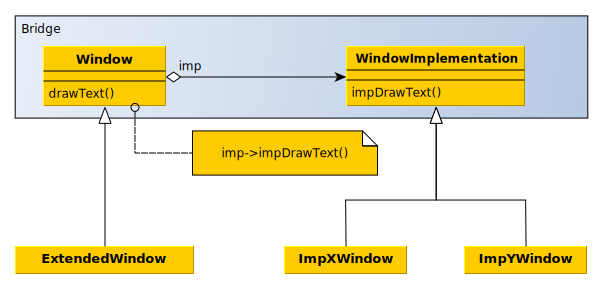
\includegraphics[width=12cm]{Immagini/BridgePattern}
\caption{Esempio di schema gerarchico dovuto all'applicazione del pattern Bridge.\label{f:bridgepattern}} 
\end{center} 
\end{figure}

L'utilizzo di questo schema permette di nascondere i dettagli implementativi ai client e di non avere effetti diretti su di esse quando l'implementazione cambia cos{\`\i} che il codice dei client non non ha un'effettiva necessit\`a di essere ricompilato. 

\subsection{Composite}
\label{sub:composite}
Lo scopo di questo pattern \`e consentire una gestione uniforme tra oggetti semplici ed oggetti compositi. Questo si traduce in una organizzazione degli oggetti in una struttura ad albero in cui ogni nodo \`e un oggetto aggregato e ogni foglia \`e un oggetto semplice.
Il nodo composito avr\`a al suo interno riferimenti ad oggetti figli che a loro volta possono essere semplici o compositi.

Spesso si desidera poter trattare oggetti composti nello stesso modo in cui gestiamo le sue componenti ignorando come siano effettivamente implementate le loro funzionalit\`a, un esempio significativo sono le interfacce grafiche in cui \`e comodo poter gestire gruppi di componenti, come pulsanti o etichette, in modo unitario come se si trattasse di una componente singola.

\begin{figure}
\begin{center}
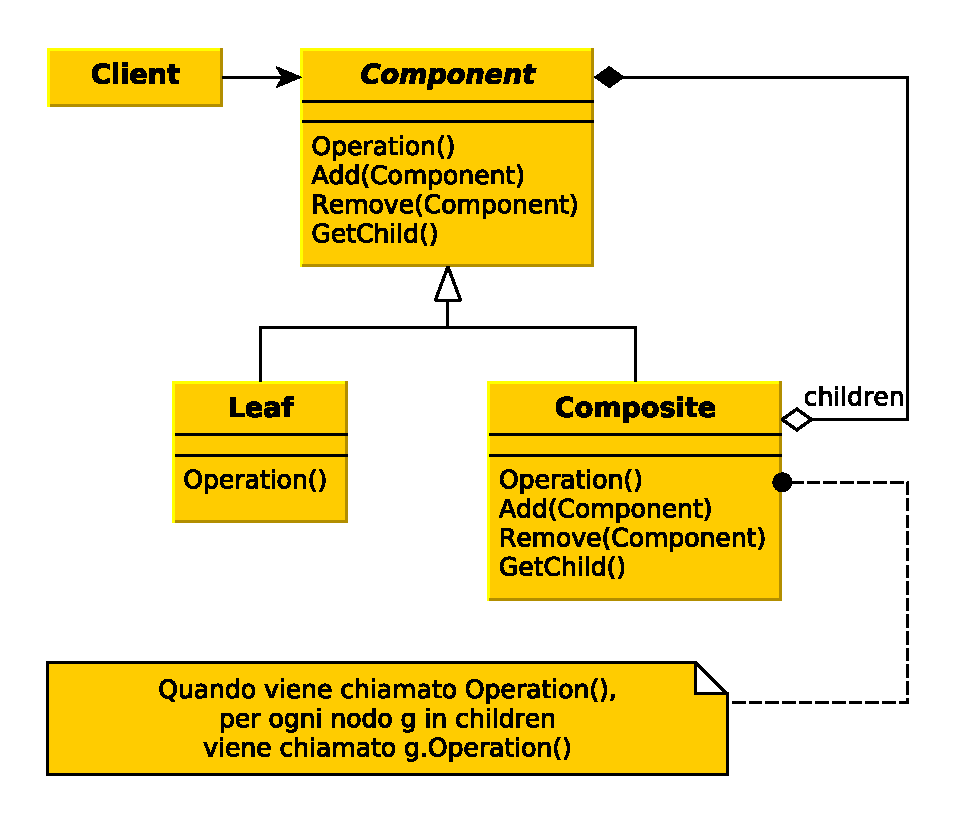
\includegraphics[width=10cm]{Immagini/CompositePattern}
\caption{Struttura UML del pattern Composite.\label{f:compositepattern}} 
\end{center} 
\end{figure}

Una metodologia per ottenere questo tipo di interazione \`e l'utilizzo di una classe astratta che rappresenti sia gli oggetti semplici, o primitive, sia gli oggetti composti, o contenitori. Nello schema \ac{UML} in figura \ref{f:compositepattern}, la classe astratta \texttt{Component} rappresenta sia oggetti foglia \texttt{Leaf} che nodi \texttt{Composite}. Un client pu\`o richiamare indifferentemente i metodi di interfaccia di un oggetto sottoclasse di \texttt{Component} sia che si tratti di un una foglia o di un nodo. Nel caso di una foglia il metodo risponder\`a direttamente in maniera appropriata mentre nel caso di un nodo verr\`a richiamato lo stesso metodo per tutti gli oggetti figli.

L'utilizzo di questo pattern consente di rendere meno complessi i moduli che utilizzano le strutture composite, che non hanno bisogno di sapere se stiano trattando una foglia o un nodo dell'albero. Consente inoltre di aggiungere in modo semplice nuovi componenti senza laboriosi interventi sul codice pre-esistente.
% TODO: valutare una citazione sul principio OpenClose SOLID


\section{Pattern Comportamentali}
I pattern comportamentali riguardano gli algoritmi e la suddivisione delle responsabilit\`a tra gli oggetti, per fare ci\`o non si limitano solamente a descrivere i rapporti tra oggetti e classi, ma anche attraverso schemi di comunicazione tra di essi. Questi schemi permettono di descrivere complessi flussi di controllo spostando l'attenzione da essi alle connessioni fra gli oggetti.

\subsection{State}
\label{sub:state}
Il pattern State ha come scopo quello di consentire ad un oggetto di cambiare il proprio comportamento durante l'esecuzione, in base alle variazioni del proprio stato interno.

Esempi di questo tipo di necessit\`a possono essere trovati in oggetti che gestiscono connessioni e che devono rispondere in modo diverso in base allo stato della connessione stessa, oppure nella costruzione di macchine a stati che implementano algoritmi di controllo.

\begin{figure}
\begin{center}
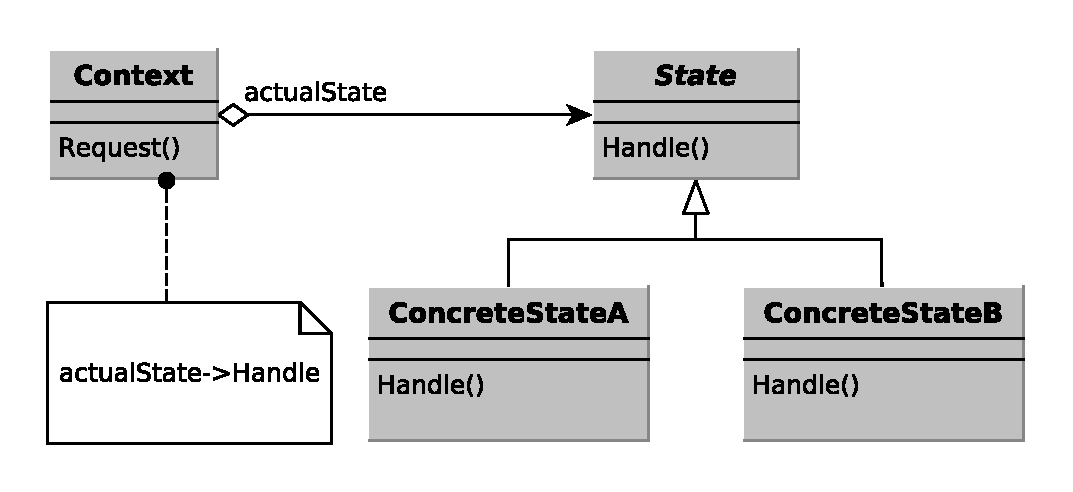
\includegraphics[width=12cm]{Immagini/StatePattern}
\caption{Schema UML del pattern State.\label{f:statepattern}} 
\end{center} 
\end{figure}

La figura \ref{f:statepattern} mostra in uno schema \ac{UML} la struttura del pattern. La classe \texttt{Context} rappresenta l'interfaccia che l'oggetto a stato variabile presenta verso i client. Al suo interno mantiene una istanza (\texttt{actualState}) di una sottoclasse concreta della classe \texttt{State}.
La classe astratta \texttt{State} definisce un'interfaccia per incapsulare il comportamento associato ad uno stato.
Le sottoclassi concrete di \texttt{State} sono associate ad un effettivo stato e implementano il comportamento che l'oggetto \texttt{Context} assume in quel caso.
Quando i client effettuano richieste all'oggetto \texttt{Context} attraverso la sua interfaccia, viene richiamato il metodo di interfaccia dell'istanza concreta \texttt{actualState}.
Il pattern non definisce dove vada inserita la logica di cambiamento di stato, ma in generale \`e pi\`u flessibile consentire alle sottoclassi di \texttt{State} la definizione dello stato successivo.

L'applicazione del pattern consente di eliminare lunghe e complesse parti di codice in cui una sequenza di istruzioni condizionali determinano le istruzioni da eseguire in base allo stato dell'oggetto. Consente inoltre di isolare il codice specifico relativo ad uno stato in un singolo oggetto permettendo l'aggiunta di nuovi stati e transizioni semplicemente definendo nuove classi.
%----------------------------------------------------------
%	Bibliografia - Varie
%----------------------------------------------------------
%\include{Varie/Bibiografia}
\bibliographystyle{plain}
\bibliography{Varie/Bibliografia}

\end{document}